\documentclass[10pt, letterpaper]{report}
% !TeX program = xelatex
%==================PREAMBOLO=======================%
\usepackage[utf8]{inputenc}
\usepackage{psvectorian}
\usepackage{pgfplots}
\usepackage[Rejne]{fncychap}
\usepackage[export]{adjustbox}
\usepackage[T1]{fontenc}
\usepackage{lmodern}
\usepackage{blindtext}
\usepackage{pdfpages}
\usepackage[shortlabels]{enumitem}
\usepackage{moresize}
\usepackage{graphicx} % Required for inserting images
\usepackage{hyperref}
\usepackage{listings}
\usepackage[table,xcdraw]{xcolor}
\usepackage{amssymb}
\usepackage{amsmath}
\usepackage[italian]{babel}
\usepackage{nicefrac, xfrac}
\usepackage{tikz}
\usepackage{tikz-3dplot}
\usepackage{mathrsfs} 
\usepackage{titletoc}
\usepackage{fancyhdr}
\usepackage{psvectorian,lipsum}
\usepackage{fourier-orns}
\usepackage{lipsum}
\usepackage{multicol}
\usepackage[paper=a4paper,left=25mm,right=25mm,bottom=25mm,top=25mm]{geometry}
\definecolor{light-gray}{gray}{0.95}
\definecolor{cop}{HTML}{f7ecd7}
\definecolor{copAut}{HTML}{ababab}
\definecolor{copAut2}{HTML}{c3c3e6}
\definecolor{purcop}{HTML}{d0d3db}
\definecolor{sapienza}{HTML}{660f1d}
\definecolor{lightSapienza}{HTML}{e3d3d5}
\definecolor{darkgreen}{HTML}{008000}
\definecolor{cartaRiciclata}{HTML}{fcfcf7}
\newcommand{\redText}[1]{\color{red}#1\color{black}}
\newcommand{\code}[1]{\colorbox{light-gray}{\texttt{#1}}}
\newcommand{\codee}[1]{\colorbox{white}{\texttt{#1}}}
\newcommand{\K}{{\mathbb K}}
\newcommand{\notimplies}{%
  \mathrel{{\ooalign{\hidewidth$\not\phantom{=}$\hidewidth\cr$\implies$}}}}
\newcommand{\flowerLine}{ \begin{center}\decofourleft\hphantom{ }\decoone\hphantom{ }\decofourright\hphantom{}\hphantom{aa}
\decofourleft\hphantom{ }\decoone\hphantom{ }\decofourright\hphantom{}\hphantom{aa}
\decofourleft\hphantom{ }\decoone\hphantom{ }\decofourright\hphantom{}\hphantom{aa}
\decofourleft\hphantom{ }\decoone\hphantom{ }\decofourright\hphantom{}\hphantom{aa} 
\decofourleft\hphantom{ }\decoone\hphantom{ }\decofourright\hphantom{}\hphantom{aa}
\decofourleft\hphantom{ }\decoone\hphantom{ }\decofourright\hphantom{}\hphantom{aa}
\decofourleft\hphantom{ }\decoone\hphantom{ }\decofourright\hphantom{}\hphantom{aa}
\decofourleft\hphantom{ }\decoone\hphantom{ }\decofourright\hphantom{}\hphantom{aa}
\decofourleft\hphantom{ }\decoone\hphantom{ }\decofourright\hphantom{}\hphantom{aa}
\end{center}}
\definecolor{g}{RGB}{60, 50, 50}
\newcommand{\textg}[1]{\color{g}{\textbf{#1}}\color{black}}
\newcommand{\teo}[1]{{\large\color{sapienza}\textbf{Teorema #1 :\hphantom{a}}}}
\newcommand{\defi}[1]{{\large\color{sapienza}\textbf{Definizione #1 :\hphantom{a}}}}
\newcommand{\claim}[1]{{\color{sapienza}\textbf{Claim #1 :\hphantom{a}}}}
\newcommand{\lemma}[1]{{\color{sapienza}\textbf{Lemma #1 :\hphantom{a}}}}
\newcommand{\dimo}[1]{{\color{sapienza}\textbf{Dimostrazione #1 :\hphantom{a}}}}
\newcommand{\prop}[1]{{\color{sapienza}\textbf{Proposizione #1 :\hphantom{a}}}}
\newcommand\greybox[1]{%
  \vskip\baselineskip%
  \par\noindent\colorbox{light-gray}{%
    \begin{minipage}{\textwidth}#1\end{minipage}%
  }%
  \vskip\baselineskip%
}
\newcommand\sapbox[1]{%
  \vskip\baselineskip%
  \par\noindent\colorbox{lightSapienza}{%
    \begin{minipage}{\textwidth}#1\end{minipage}%
  }%
  \vskip\baselineskip%
}
\newcommand{\ridFunc}{{f:\Sigma^*\rightarrow \Sigma^*}}
\newcommand{\rid}{{\le_m^P}}
\newcommand{\Z}{{\mathbb Z}}
\newcommand{\blank}{{\sqcup}}
\newcommand{\R}{{\mathbb R}}
\newcommand{\N}{{\mathbb N}}
\newcommand{\C}{{\mathbb C}}
\newcommand{\Sn}{{\mathcal S_n}}
\newcommand{\An}{{\mathcal A_n}}
\newcommand{\E}{{\mathcal E}}
\newcommand{\B}{{\mathcal B}}
\newcommand{\mcm}{{\text{mcm}}}
\newcommand{\rg}{{\text{rg}}}
\newcommand{\ve}{{\bar v}}
\newcommand{\spaz}{{\text{\hphantom{aa}}}}
\newcommand{\MCD}{{\text{MCD}}}
\newcommand{\tc}{{\text{ tale che }}}
\newcommand{\supp}{{\text{Supp}}}
\newcommand{\acc}{\\\hphantom{}\\}
\newcommand{\esempio}[1]{{\acc\large\color{sapienza}\textbf{Esempio #1 \hphantom{a}}\acc}}
\newcommand{\bra}[1]{\langle #1 \rangle}
\newcommand{\aut}{{\text{Aut}}}
\newcommand{\Span}{{\text{Span}}}
\newcommand{\End}{{\text{End}}}
\newcommand{\cen}{{\text{Centro}}}
\newcommand{\norm}{{\unlhd}}
\newcommand{\ciclS}{{\left \langle }}
\newcommand{\ciclE}{{\right \rangle }}
\newcommand{\boxedMath}[1]{\begin{tabular}{|c|}\hline \texttt{#1} \\ \hline\end{tabular} :} 
\newcommand{\shell}[1]{\colorbox{black}{\textcolor{white}{\texttt{#1}}}}
\newcommand{\eqImportante}[1]{\begin{center}\huge\lefthand\hphantom{a}
    \normalsize\texttt{#1}
    \hphantom{aaa}\huge\righthand\end{center}}

\fancyhf{}
\pagestyle{fancy}
\usepackage{pgf-pie}  
\usetikzlibrary{positioning}

\renewcommand{\headrule}{%
\vspace{-8pt}\hrulefill
\raisebox{-2.1pt}{\quad\decothreeleft\decotwo\decothreeright\quad}\hrulefill}

%sta roba serve per il codice C
\definecolor{mGreen}{rgb}{0,0.6,0}
\definecolor{mGray}{rgb}{0.5,0.5,0.5}
\definecolor{mPurple}{rgb}{0.58,0,0.82}
\definecolor{backgroundColour}{rgb}{0.95,0.95,0.92}

\lstdefinestyle{CStyle}{
    backgroundcolor=\color{backgroundColour},   
    commentstyle=\color{mGreen},
    keywordstyle=\color{magenta},
    numberstyle=\tiny\color{mGray},
    stringstyle=\color{mPurple},
    basicstyle=\footnotesize,
    breakatwhitespace=false,         
    breaklines=true,                 
    captionpos=b,                    
    keepspaces=true,                 
    numbers=left,                    
    numbersep=5pt,                  
    showspaces=false,                
    showstringspaces=false,
    showtabs=false,                  
    tabsize=2,
    language=C
}
\lstdefinestyle{CppStyle}{
    backgroundcolor=\color{backgroundColour},   
    commentstyle=\color{mGreen}\ttfamily,
    morecomment=[l][\color{magenta}]{\#}
    keywordstyle=\color{blue}\ttfamily,
    numberstyle=\tiny\color{mGray},
    stringstyle=\color{red}\ttfamily,
    basicstyle=\ttfamily,
    breakatwhitespace=false,         
    breaklines=true,                 
    captionpos=b,                    
    keepspaces=true,                 
    numbers=left,                    
    numbersep=5pt,                  
    showspaces=false,                
    showstringspaces=false,
    showtabs=false,                  
    tabsize=2,
    language=C
}
\lstset{language=C++,
                basicstyle=\ttfamily,
                keywordstyle=\color{blue}\ttfamily,
                stringstyle=\color{red}\ttfamily,
                commentstyle=\color{green}\ttfamily,
                morecomment=[l][\color{magenta}]{\#}
}
%fine roba che serve per il codice C
\usepackage{minted}
\usepackage{circuitikz}
\ctikzset{bipoles/thickness=1.2}

\newcommand{\midlabelline}[3]{
   \node (midlabel) at ($ (#1)!.5!(#2) $) {#3};
   \draw[latex-] (#1) --  (midlabel);
   \draw[-latex] (midlabel) -- (#2);
}
\usetikzlibrary{petri}
 %TOGLI COMMENTO SE USI XELATEX
%\usepackage{fontspec}
\title{\jobname} %========TITOLO========%
\author{Marco Casu}
\date{\vspace{-5ex}}
\begin{document}

%==================COPERTINA=======================%
\begin{titlepage}
    \pagecolor{copAut}
\begin{center}
    %TOGLI COMMENTO SE USI XELATEX
   %\setmainfont{Palace Script MT}
   \HUGE Marco Casu\acc
    %\setmainfont{Grand Casino}
     %TOGLI COMMENTO SE USI XELATEX
    %\setmainfont{h Halfroad}
    \HUGE \decothreeleft\hphantom{ }{\fontsize{48}{50}\selectfont \jobname}\hphantom{ }\decothreeright
     %TOGLI COMMENTO SE USI XELATEX
   % \setmainfont{Times New Roman}
\end{center}
\thispagestyle{empty}
\begin{figure}[h]
    \centering{
        %l'immagine deve avere una risoluzione 2048x2048
        \includegraphics[width=1\textwidth ]{images/Copertina.jpeg}
    }
\end{figure}
\vfill 
\centering \includegraphics[width=0.4\textwidth ]{../../../preamble/Stemma_sapienza.png} \acc
\centering \Large \color{sapienza}Facoltà di Ingegneria dell'Informazione,
Informatica e Statistica\\
Dipartimento di Informatica
\end{titlepage}

%===================FINE COPERTINA======================%
\newpage
\pagecolor{cartaRiciclata}%\setmainfont{Algerian}
\Large
Questo documento è distribuito sotto la licenza 
\color{blue}\href{https://www.gnu.org/licenses/fdl-1.3.txt}{GNU}\color{black},  
è un resoconto degli appunti (eventualmente integrati con libri di testo) tratti dalle lezioni del corso di \jobname
\hphantom{a}per la laurea 
triennale in Informatica. Se dovessi notare errori, ti prego di segnalarmeli.\acc 
Nota bene : Essendo questi appunti di un corso esterno alla facoltà di Informatica, 
è presente un capitolo "Complementi" che può risultare utile al lettore.
\vfill
\begin{figure}[h!]
    \raggedright
    \includegraphics[width=0.4\textwidth,right ]{../../../preamble/tomodachi.pdf} 
\end{figure}
\newpage %\setmainfont{Times New Roman}
\normalsize
\tableofcontents 
\newpage

%==================FOOTER e HEADER=======================%
\fancyhf{}
\fancyhead[L]{\nouppercase{\leftmark}}
\fancyhead[R]{Sezione \thesection}
\fancyfoot[C]{\thepage}
\fancyfoot[L]{Appunti di \jobname}
\fancyfoot[R]{ Marco Casu}
%\fancyfoot[R]{\setmainfont{Palace Script MT}\huge Marco Casu \setmainfont{Times New Roman}}
%==================FOOTER e HEADER=======================%

%Ricorda del comando \flowerLine per separare le sottosezioni. Le sezioni si separano nelle diverse pagine

%==================INIZIO======================%
\chapter{L'Automazione Industriale}
\section{Introduzione}
Con il termine \textit{Automazione}, si intende la trasformazione 
di un processo pre-esistente, al fine di renderlo autonomo, riducendo o 
sostituendo del tutto l'intervento umano, verrà trattata l'automazione 
dei processi industriali e manifatturieri, e del loro controllo e 
supervisione. I sistemi presi in considerazione evolvono nel 
tempo e reagiscono ad eventi, che ne cambiano lo stato, e scaturiscono 
dei feedback, per un eventuale correzione dell'errore.\acc 
Con sistema \textit{autonomo} si intende un sistema in cui viene 
ridotto l'intervento umano. L'\textit{Automatica} si occupa di 
sfruttare gli strumenti dell'informatica per l'automazione, acquisendo informazioni 
dal mondo fisico tramite appositi sensori, per poi essere elaborate 
su un sistema di controllo (calcolatore), o una rete di calcolatori, 
che implementa dei protocolli standard per l'industria. Differentemente da 
altri contesti, come la trasmissione (ad esempio, di un video in streaming) nelle 
reti dell'automazione i ritardi risultano critici, e vanno ridotti al 
minimo.
\begin{center}
    \begin{figure}[h!]
        \centering
        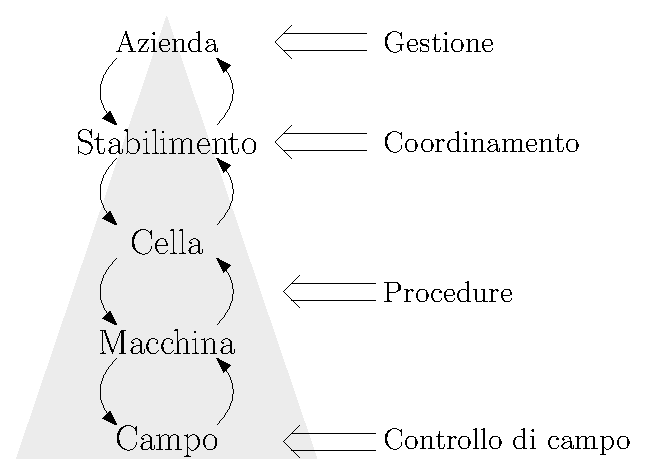
\includegraphics[width=0.4\textwidth ]{images/CIM.eps}
        \caption{Piramide CIM}
        \label{fig:cim}
   \end{figure}
   \end{center}
La \textit{piramide CIM}, mostrata in figura \ref{fig:cim}
schematizza la gestione di un processo industriale e delle sue procedure, 
ogni strato comunica con quelli adiacenti scambiandosi informazioni, nei 
livelli più alti, le informazioni sono più \textit{raffinate} ed 
astratte, nei livelli più bassi sono più grezze, ad esempio\begin{itemize}
    \item Al livello azienda viene decisa la produzione di un articolo (che 
    coinvolgerà l'utilizzo di un braccio robotico)
    \item Al livello macchina, l'informazione che arriverà al braccio 
    sarà semplicemente relativi ai gradi in cui i suoi giunti devono 
    ruotare
    \item Al livello di campo, l'informazione comprenderà semplicemente 
    il voltaggio da applicare alla macchina in questione per avere l'effetto 
    desiderato.
\end{itemize}
Con \textbf{cella}, si intende un unità composta da più macchine, in 
cui viene scambiato e lavorato del materiale per compiere delle azioni,
il \textit{controllo delle procedure} si occupa delle \textbf{macchine}, ed uno 
\textbf{stabilimento} è un complesso di celle/parti e catene 
di montaggio. nel livello di campo, vengono utilizzati vari dispositivi, 
quali\begin{itemize}
    \item motori elettrici, servomotori, encoder 
    \item azionatori di valvole, dynamo tachimetrici, sensori di temperatura
\end{itemize}
Tali sensori presenteranno stesso un comportamento lineare, ad esempio, 
se una tensione $x$ causa una rotazione di $y$ giri per minuti, allora 
una tensione $2x$ causerà una  rotazione di $2y$. Anche se tali dispositivi 
non si prestano ad un comportamento lineare, ne verrà causata una volontaria 
linearizzazione, correggendone il comportamento.\acc 
Argomento centrale saranno i regolatori \textit{PID}, la cui definizione, 
come molte altre trattate in questo capitolo, sarà ripresa ed 
approfondita in seguito. tali regolatori agiscono su delle grandezze 
di campo.\begin{center}
    \begin{figure}[h!]
        \centering
        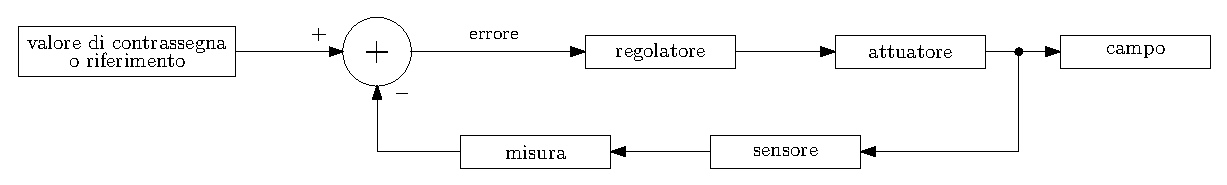
\includegraphics[width=1\textwidth ]{images/schemaPID.eps}
        \caption{schematizzazione del regolatore PID}
        \label{fig:schemaPID}
   \end{figure}
\end{center}
Si consideri il seguente esempio di regolatore, vi è una stufa che deve 
riscaldare una stanza, ed un sensore che ne misura la temperatura, il valore 
da raggiungere, detto \textit{setpoint}, è di 20 gradi celcius. Si supponga che il 
sensore, una volta rilevata la temperatura, debba accendere e spengere la stufa 
in modo che si raggiunga la temperatura adeguata.
\begin{center}
    \begin{figure}[h!]
        \centering
        \includegraphics[width=0.6\textwidth ]{images/stufaEsempio.eps}
        \caption{Azioni sulla stufa}
        \label{fig:stufa}
   \end{figure} 
\end{center}
In figura \ref{fig:stufa}, il differenziale rappresenta un margine 
di differenza rispetto il setpoint, quando la temperatura è 
sotto il limite inferiore, la stufa viene accesa, quando è oltre il limite 
superiore, viene spenta (è chiaro che la velocità con la quale la temperatura 
cambia dipende dalle capacità della stufa e dalla dispersione del calore nella stanza).\acc 
Ridurre il valore del differenziale costringerebbe la temperatura ad assestarsi 
sempre di più sul valore desiderato, ma ciò, comporterebbe un'accensione/spengimento della 
stufa più frequente, aumentando lo \textit{sforzo di controllo}, è quindi, in questo 
caso, accettabile un differenziale di $2^\circ$.\acc 
Tale modello di controllo è il più semplice che ci sia, esistono ovviamente altri modi di regolare un 
segnale in modo che esso raggiunga il valore desiderato, ad esempio, calcolare l'errore $e$ (ossia la differenza 
fra il valore desiderato ed il valore effettivo) e scalarlo ad una certa costante $K_p$ per poi utilizzare tale 
valore nella regolazione del segnale.
\begin{center}
    \begin{figure}[h!]
        \centering
        \includegraphics[width=0.6\textwidth ]{images/stufaEsempioPROP.eps}
        \caption{Regolatore proporzionale}
        \label{fig:regPropStuda}
   \end{figure} 
\end{center}
Anche se la variazione della temperatura è continua nel tempo, il suo 
superare una certa soglia è un evento, i PLC (controllori logici programmabili) 
agiscono sulle misure di campo, un noto linguaggio utilizzato per descriverne 
il funzionamento è noto come \textit{Sequential Flow Chart (SFL)}.\acc 
Nei sistemi di automazione industriale vengono prediletti controllori e sensori distribuiti piuttosto 
che centralizzati, se ne vuole dare una dimostrazione pratica con il segunete 
esempio : Si considerino i due seguenti modi per trasportare un oggetto 
su un nastro trasportatore :\begin{center}
    \begin{figure}[h!]
        \centering
        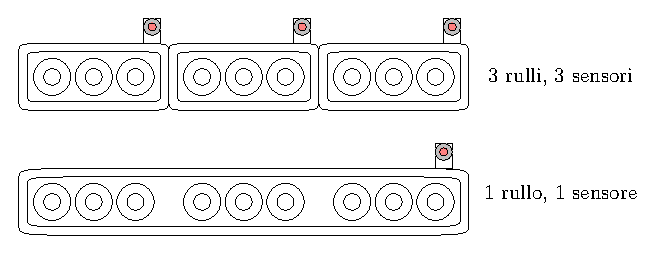
\includegraphics[width=0.6\textwidth ]{images/rulli.eps}
        \caption{Rulli}
        \label{fig:rulli}
   \end{figure} 
\end{center}
Ogni nastro ha un sensore, se un oggetto è rilevato sopra il nastro, allora il motore si attiva. Risulta più efficente 
la soluzione con 3 nastri in quanti sarà adoperata solamente la zona del nastro in cui è rilevato l'oggetto, piuttosto 
che l'intero nastro.\acc 
Per la modellizzazione di sistemi autonomi verranno adoperati automi a stati finiti, ampiamente trattati nel 
corso di 
\color{blue}\href{https://github.com/CasuFrost/University_notes/blob/main/Terzo%20Anno/Automi%2C%20Calcolabilit%C3%A0%20e%20Complessit%C3%A0/Automi%2C%20Calcolabilit%C3%A0%20e%20Complessit%C3%A0.pdf}{Automi, Calcolabilità e Complessità}
\color{black}, e \textit{Reti di Petri}. Una rete di Petri, non è altro che un grafo bipartito, in cui ogni nodo 
appartiene ad un'insieme fra \begin{itemize}
    \item nodi \textit{posto}
    \item nodi \textit{transizione}
\end{itemize}
Inoltre, i nodi posto possono essere annotati con dei pallini neri, detti \textit{token}, essi rappresentano 
lo stato del sistema in quanto indicano che delle risorse (in senso generale) sono disponibili in un posto, 
permettendo eventualmente una transizione. Ogni arco del grafo collega un nodo posto ad un nodo transizione.
\begin{figure}[h!]
    \centering
    \begin{tikzpicture}
        \node[place,tokens=2,label=above:$p_1$]        (p1) {};
        \node[place,label=above:$p_2$,right=of p1] (p2) {};
        \node[place,tokens=1,label=above:$p_3$,right=of p2] (p3) {};
        \node[place,label=above:$p_4$,below=of p3,right=of p3] (p4) {};
        \node[place,tokens=1,label=above:$p_5$,below=of p1] (p5) {};
       
      
        \node[transition,below right=of p1,label=below:$t_1$] {}
          edge[pre]                 (p1)
          edge[post] node[auto] {} (p2)
          edge[post] node[auto] {} (p5);
        \node[transition,below right=of p2,label=below:$t_2$] {}
          edge[pre]                 (p2)
          edge[post] node[auto] {} (p3)
          edge[post] node[auto] {} (p4);
      \end{tikzpicture}
      \caption{Esempio di una rete di Petri}
\end{figure}\acc
Le macchine per l'automazione possono essere di vari tipi, ad esempio, comprendere un unico attuatore, e più 
meccanismi di attuazione del moto che utilizzano una sola fonte. Un altro tipo di macchine sono quelle 
a \textit{controllo numerico}, macchine programmate per fare compiti elementari periodicamente. \acc 
Quando in un processo produttivo il materiale viene trasformato in maniera continuativa (come nell'industria 
farmaceutica o alimentare) si parla di \textbf{produzione continua}. Nel caso in cui i materiali sono processati 
in quantità finite e determinate si parla di \textbf{produzione a lotti}, le pause dovute fra la lavorazione di un lotto 
e l'altro sono dovute al fatto 
che è necessario trasformare solo una determinata quantità di materiale grezzo.\acc 
L'automazione industriale fa largo utilizzo dei \textit{robot}, bracci meccanici che presentano diversi 
gradi di libertà, ossia giunti, che possono ruotare attorno un certo asse. 
   \begin{center}
	\begin{tabular}{>{\centering\arraybackslash}m{3in}>{\arraybackslash}m{3in}}
        \includegraphics[width=0.3\textwidth ]{images/braccioRobot.pdf} & L'organo terminale, posto alla fine 
        del braccio (in un certo senso, la sua "mano"), può assumere una certa configurazione (posizione e direzione) a 
        seconda della rotazione di ogni giunto del braccio. 
        Si può dire che la posizione finale $p$ e la sua direzione sono in funzione degli angoli 
        $\theta_1,\theta_2\dots,\theta_n$ di rotazione di ogni giunto.
		\\
	\end{tabular}
\end{center}
La procedura di comando da far eseguire al robot si traduce in una funzione nel tempo che descrive in che modo 
deve variare la rotazione di ogni singolo giunto, quest'ultima al livello di campo, si traduce nell'attuazione 
dei motori elettrici posti sui giunti.
\begin{center}
        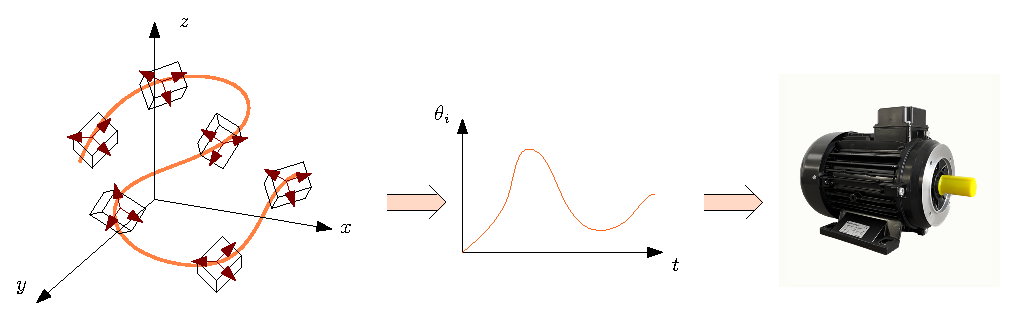
\includegraphics[width=1\textwidth ]{images/rotBraccioRobot.eps}
\end{center}
Altri tipi di macchine per la movimentazione oltre i robot sono i rulli o i carrelli automatici, questi ultimi 
inizialmente potevano muoversi seguendo un percorso stabiliti da magneti posti sul terreno, vengono dotati di 
sensori di prossimità per evitare collisioni. I carrelli moderni non sono limitati da percorsi prestabiliti, sono 
autonomi e possono fare percorsi arbitrari, che vengono calcolati da un elaboratore che ha la "visione" completa 
di essi.\acc 
Sorge spontaneo chiedersi quale sia la differenza fra Automazione e Robotica.\begin{itemize}
    \item \textit{Analogie} : Entrambe coinvolgono l'informatica ed i calcolatori, interfacciandosi con il mondo 
    fisico, entrambe sfruttano conoscenze e tecnologie multi-disciplinari. 
    \item \textit{Differenze} : La robotica mostra la fattibilità di una soluzione, l'automazione si occupa di 
    porsi delle domande riguardo tale soluzione, fra cui l'efficenza, l'ottimalità, la fattibilità e l'affidabilità.
\end{itemize}
Formalmente, si definisce \textbf{processo} la \textit{trasformazione} di \textit{materiali} in 
\textit{prodotti}. Tale trasformazione richiede 
\begin{itemize}
    \item Energia 
    \item Informazione 
    \item Controllo
\end{itemize}
Anche la costruzione di uno strumento per la caccia da parte di un uomo primitivo è un processo, in quel caso, 
l'energia è data dai muscoli del corpo, l'informazione viene dai sensi, quali vista e tatto, ed il controllo 
avviene da parte del cervello.
\begin{center}
    \includegraphics[width=0.5\textwidth ]{images/caveMan.eps}
\end{center}
Lo scopo dell'automazione nel tempo è stato quello di sostituire o eliminare l'intervento dell'uomo 
nei processi, spesso è faticoso e pericolo fornire energia, e l'uomo non ha le capacità sufficienti per 
gestire in maniera precisa l'informazione ed il controllo.\acc 
Il \textbf{primo passo} di industrializzazione è stato quello di sostituire l'energia fornita dall'uomo con l'energia 
naturale ed animale, durante la prima rivoluzione industriale, dove la produzione dipendeva da macchine 
azionate tramite potenza meccanica derivante da fonti energetiche come mulini.\acc 
Il \textbf{secondo passo} riguarda la sostituzione delle operazioni di controllo, un importante esempio fu il 
\textit{regolatore di velocità} di Watt (1785), fu la prima applicazione di regolatore automatico, e sfruttava 
la forza centrifuga di due masse in rotazione per regolare la velocità di una macchina a vapore.
\begin{figure}[h!]
    \centering
    \includegraphics[width=0.4\textwidth ]{images/watt.pdf}
    \caption{regolatore di Watt}
    \label{fig:watt}
\end{figure} \acc
Il funzionamento è semplice, il vapore passante per la valvola fa aumentare la velocità di rotazione del 
regolatore, per la forza centrifuga, le masse poste sulla valvola a farfalla si allontanano, alzandosi, 
qui la gravità oppone resistenza facendo chiudere la valvola essendo che le masse tendono ad avvicinarsi al 
suolo, facendone diminuire la velocità di rotazione.  
Tali automatismi sono compresi dalla teoria dei controlli automatici, che definisce l'azione di comando più efficace 
per ottenere il comportamento desiderato a seguito di una certa misurazione fisica.\acc
Il \textbf{terzo passo} riguarda la gestione delle informazioni mediante sistemi combinatorici/sequenziali che al 
verificarsi di determinate condizioni reagiscono con operazioni di base. La prima generazione di controllori 
prevedeva circuiti elettronici composti da bobine e relé, essi erano ingombranti e lenti nell'acquisizione 
delle informazioni, inoltre la loro logica era prestabilita e ridefinirla scaturiva una modifica sostanziale 
del circuito. \acc 
Con l'avvento dei semiconduttori si è introdotta la seconda generazione di controllori, basati su schede 
elettroniche stampate, riducendo i costi ed aumentando l'efficenza, non risolvendo però il problema della bassa 
flessibilità, in quanto tali schede erano progettate per gestire una specifica logica. \acc 
La terza generazione di controllori vede i microprocessori protagonisti, grazie all'evoluzione dell'elettronica 
e dell'informatica sono ad oggi utilizzabili schede riprogrammabili (PLC) altamente flessibile, capaci di eseguire 
un generico algoritmo logico sequenziale.
\begin{center}
    \begin{tabular}{|c|c|c|}
        \hline
        \rowcolor[HTML]{6665CD} 
        {\color[HTML]{FFFFFF} Rivoluzione Industriale} & {\color[HTML]{FFFFFF} Periodo Temporale} & {\color[HTML]{FFFFFF} Tecnologie e Caratteristiche}                                                                                                                                                                                                                                                                                                                               \\ \hline
        \rowcolor[HTML]{DAE8FC} 
        prima                                          & 1785 – metà 19° secolo                   & \begin{tabular}[c]{@{}c@{}}utilizzo di macchine azionate da energia\\  meccanica (vapore, acqua)\end{tabular}                                                                                                                                                                                                                                                                     \\ \hline
        \rowcolor[HTML]{F2F7FE} 
        seconda                                        & fine 19°secolo – 1970                    & \begin{tabular}[c]{@{}c@{}}azionamento elettrico delle macchine e produzione\\  di massa basata sulla\\  divisione del lavoro (catene di montaggio)\end{tabular}                                                                                                                                                                                                                  \\ \hline
        \rowcolor[HTML]{DAE8FC} 
        terza                                          & 1970 – oggi                              & \begin{tabular}[c]{@{}c@{}}utilizzo dell’elettronica e delle tecnologie\\  del’informazione (IT) \\ per aumentare il livello di automazione di attività\\  complesse (CNC, robot e computer)\end{tabular}                                                                                                                                                                         \\ \hline
        \rowcolor[HTML]{F2F7FE} 
        quarta                                         & oggi – futuro                            & \begin{tabular}[c]{@{}c@{}}sviluppo di macchine sensorizzate e intelligenti,\\  interconnesse tra loro e con internet, con la raccolta,\\  analisi e uso di grandi \\ quantità di informazioni (Big data), per una\\  specializzazione di \\ massa del prodotto, l’integrazione della\\  catena produttiva \\ (supply and value chains) e una maggiore\\  efficenza\end{tabular} \\ \hline
        \end{tabular}
\end{center}
\flowerLine
\section{Processi Industriali}
I sistemi di produzione automatizzati sono composti da 
diverse componenti\begin{itemize}
    \item processo produttivo - movimentazioni meccaniche, attuazioni, 
    trasformazioni fisiche e chimiche 
    \item sistema di controllo - uno o più dispositivi messi in comunicazione 
    con il processo produttivo, potendo agire su di esso riducendo 
    l'intervento umano. 
    \item impianto di produzione - macchinari, edifici, componenti
\end{itemize}
Si considerino i seguenti esempi di produzione industriale\begin{itemize}
    \item \textbf{produzione di energia elettrica} \begin{itemize}
        \item materie prime (input continuo) : combustibile fossile, ossigeno 
        \item prodotto (output continuo) : energia elettrica misurata in Kilowatt/ore
        \item impianto necessario : tubature, caldaia, turbine, bruciatori, pompe, valvole, camini, edifici di
        sostegno e di contenimento, sensori
        
    \end{itemize}
    \item \textbf{produzione di vernice} \begin{itemize}
        \item materie prime (input continuo) : resine, coloranti, acqua, additivi
        \item prodotto (output discreto) : barattoli di vernice
        \item impianto necessario : reattori (dove avvengono le reazioni principali), miscelatori, riscaldatori,
        tubature, pompe, valvole, edificio di sostegno e di contenimento, sensori
    \end{itemize}
    \item \textbf{produzione di parti meccaniche di motori} \begin{itemize}
        \item materie prime (input discreto) : pezzo metallico grezzo
        \item prodotto (output discreto) : componenete del motore
        \item impianto necessario : macchina con mandrini per la meccanica (fresatura, foratura, ...), sistema di
        controllo numerico (posizionamento corretto dell’utensile del mandrino),
        dispositivo di cambio utensile automatico, protezioni, sistemi di scarico
        trucioli
    \end{itemize}
\end{itemize}
\subsection{Sistema di Controllo}
Il sistema di controllo interagisce con il processo 
attraverso \textit{sensori} e \textit{trasduttori}. Acquisiscono 
informazioni dal mondo fisico (pressione, temperatura) e le convertono in segnali 
facilmente analizzabili e controllabili (segnali elettrici).
\acc 
Un esempio di sensore per misurare la forza, consiste in un circuito il cui
resistore viene deformato quando rilevata una pressione sul sensore, 
variandone la resistenza.\acc 
Una volta raccolte le informazioni, è possibile cambiare le variabili 
di controllo del processo per ottenere il comportamento desiderato. Solitamente, 
il segnale di controllo è a bassa potenza, non sufficiente per correggere il comportamento 
di grossi attuatori, a tal proposito sono adoperati gli \textit{amplificatori}. Le informazioni 
sono elaborate da un apposito calcolatore che può essere inglobato o 
esterno alla macchina in questione.\acc
Nei sistemi di controllo è stata definita una normativa, nota come 
IEC61499 per normalizzare il funzionamento generale di tali 
dispositivi. In particolare, deve un sistema di controllo deve 
rifarsi ai seguenti punti\begin{itemize}
    \item è un sistema informatico che elabora informazioni ed 
    esegue/applica algoritmi.
    \item è costituito da vari dispositivi che comunicano attraverso un'apposita 
    rete. 
    \item i dispositivi devono implementare delle funzionalità, denominate \textit{applicazioni}.
    \item tali applicazioni possono essere distribuite fra i vari dispositivi. 
    \item i dispositivi devono interfacciarsi con la rete e con il processo, 
    inoltre le applicazioni costituiscono le loro \textit{risorse}.
    \item in particolare, una \textit{risorsa} è costituita da\begin{itemize}
        \item una o più applicazioni 
        \item funzioni che collegano dati ed eventi 
        \item funzioni di pianificazione delle attività (un sistema operativo)
    \end{itemize}
\end{itemize}
\begin{figure}[h!]
    \centering
    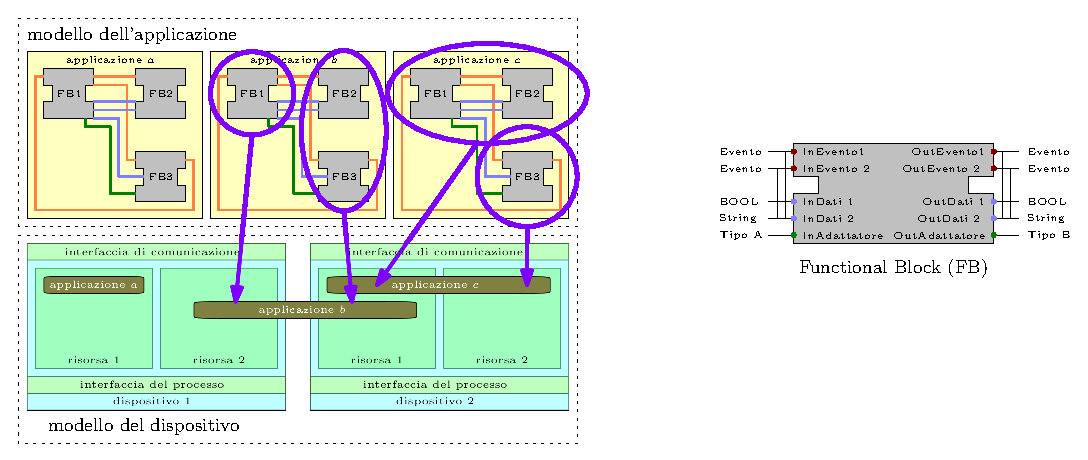
\includegraphics[width=1\textwidth ]{images/sistemaControllo.eps}
    \caption{schematizzazione di un sistema di controllo}
    \label{fig:siscon}
\end{figure} 
Si definisce \textbf{Manifacturing} l'insieme dei processi 
produttivi da applicare per ottenere un prodotto finale desiderato, a partire 
da materiali grezzi. Richiede \begin{itemize}
    \item energia 
    \item macchine 
    \item intervento umano 
    \item informazioni
\end{itemize}
Da un punto di vista economico, è il processo che da valore aggiunte 
ai materiali utilizzati.\begin{center}
    \includegraphics[width=0.7\textwidth ]{images/manifacturing.eps}
\end{center}
Spesso di questi processi produttivi ce ne sono molteplici messi a catena, in modo che l'output di un 
processo sia l'input di un altro. Si consideri il seguente esempio che schematizza un sistema di produzione del cemento.
\begin{figure}[h!]
    \centering
    \includegraphics[width=0.7\textwidth ]{images/cementificio.pdf}
    \caption{Cementificio : schema}
    \label{fig:cementificio}
\end{figure} 
Il cemento viene prodotto a partire da calcari pure ed argilla, viene mandato nel frantoio per essere 
tritati, ciò che ne esce viene miscelato per poi venire accumulato in un silos. Quest'ultimo, funge 
da \textit{buffer}, ossia un accumulo del prodotto non ancora terminate durante la sequenza di produzione, utile 
nel sincronizzare la catena, qui 
viene riempito totalmente prima di passare allo step successivo. Il primo mulino esegue una fase 
di pre riscaldamento, il calore utilizzato deriva dall'energia termica scartata dal forno principale 
ad alte temperature. \acc 
Il processo consiste in una \textit{sequenza} di \textit{operazioni elementari} di varia natura \begin{itemize}
    \item lavorazione  e assemblaggio
    \item trasporto e stoccaggio 
    \item verifica, test, e coordinamento
\end{itemize}
Fin'ora è stato evidenziato se le materie prime o il prodotto finale di un certo processo fossero 
numerabili oppure no, a tal proposito, è possibile classificare i processi produttivi nel seguente 
modo
\begin{center}
    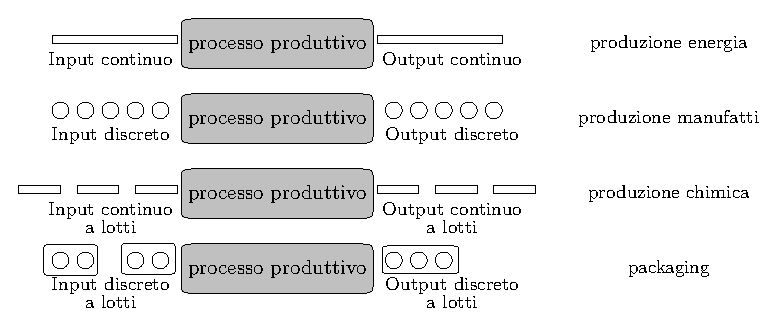
\includegraphics[width=0.7\textwidth ]{images/classificazioneProcProd.eps}
\end{center}
\begin{itemize}
    \item\textbf{processi continui} : Trattano la trasformazione continua nel tempo della materia, energia 
    e quantità di moto. L'obiettivo è mantenere uniforme nel tempo la qualità del prodotto, gli scambi 
    avvengono sulle variabili fisiche.
    \item\textbf{processi a lotti} : Possono essere sia continui che discreti, il prodotto finale necessita 
    di una specifica, e finita, quantità di materia prima per essere prodotto. Segue una specifica 
    sequenza di lavorazione detta \textit{ricetta}, il processo si intorrempo fra un lotto ed un 
    altro. Obbiettivo dell'automazione è la definizione delle ricette, garantire un uso corretto delle 
    risorse e realizzare tale sistemi in modo che siano ripetibili.
    \item\textbf{processi semi continui} : \redText{TODO} 
    \item \textbf{processi discreti} : Si lavora su singoli prodotti, materiali numerabili, è una 
    produzione tipica dell'industria manifatturiera.
\end{itemize}
I sistemi di controllo dei processi prevedono azioni di tipo \textit{logico} oppure \textit{diretto}\begin{center}
    \begin{tabular}{
        >{\columncolor[HTML]{ECF4FF}}c |
        >{\columncolor[HTML]{FFFFFF}}c |
        >{\columncolor[HTML]{FFFFFF}}c |}
        \cline{2-3}
        \cellcolor[HTML]{FFFFFF}                                        & \cellcolor[HTML]{ECF4FF}Controllo logico                                                                                                                                    & \cellcolor[HTML]{ECF4FF}Controllo diretto                                                                                                                                           \\ \hline
        \multicolumn{1}{|c|}{\cellcolor[HTML]{ECF4FF}Processi continui} & \begin{tabular}[c]{@{}c@{}}coordinamento complessivo\\  avviamento\\  e spegnimento guasti e emergenze\end{tabular}                                                         & \begin{tabular}[c]{@{}c@{}}controlli primari \\ (livelli, temperature, pressioni)\\  controlli asserviti (portata pompe, \\ posizione valvole)\end{tabular}                         \\ \hline
        \multicolumn{1}{|c|}{\cellcolor[HTML]{ECF4FF}Processi a lotti}  & \begin{tabular}[c]{@{}c@{}}controllo delle ricette\\  supervisione impianto\\  avviamento e  spegnimento guasti\\  e emergenze \\ allocazione risorse impianto\end{tabular} & \cellcolor[HTML]{FFFFFF}\begin{tabular}[c]{@{}c@{}}controlli primari (livelli,\\  temperature, pressioni)\\  controlli asserviti (portata pompe, \\ posizione valvole)\end{tabular} \\ \hline
        \multicolumn{1}{|c|}{\cellcolor[HTML]{ECF4FF}Processi discreti} & \begin{tabular}[c]{@{}c@{}}controllo sequenze di lavoro \\ delle singole macchine \\ supervisione impianto \\ avviamento e spegnimento \\ guasti e emergenze\end{tabular}   & \begin{tabular}[c]{@{}c@{}}controlli asserviti (posizionamento,\\  velocità \\ motori elettrici)\end{tabular}                                                                       \\ \hline
        \end{tabular}
\end{center}
\begin{itemize}
    \item \textit{regolazione} : Portare un segnale ad un determinato valore di riferimento 
    \item \textit{asserimento} : Far si che il segnale segua una certa dinamica nel tempo
\end{itemize}
Il \textit{controllo diretto} riguarda il rilevamento di grandezze fisiche analogiche da parte di 
sensori posti sul campo, tali valori continui nel tempo vengono 
convertiti in segnali digitali, confrontandoli poi con il valore di riferimento, dando l'azione di comando 
per correggere il comportamento delle variabili.\begin{enumerate}
    \item I sensori forniscono un segnale \textbf{analogico} $x(t)$ continuo nel tempo (temperatura, posizione)
    \item Tale segnale viene \textbf{quantizzato}, denotato $x_q(t)$, costringendolo ad assumere un numero limitato di 
    valori prestabiliti $\Delta$, separati da un ampiezza $q$, il numero di bit necessari 
    a rappresentare i valori del segnale sarà $n=\log_{2}(\nicefrac{\Delta}{q})$
    $$ x_q(t)=\lfloor\frac{x(t)}{q}\rfloor\cdot q$$
    \item Il segnale analogico quantizzato viene poi \textbf{campionato}, ossia, viene valutato 
    eslcusivamente in determinati intervalli di tempo separati da un tempo di campionamento $T_C$ 
    $$x_q(t) \longrightarrow  x_q(kT_C)\ \ \ \ t\in\R \ \ k\in\mathbb{Z}$$
    \item A tal punto si ha un \textbf{segnale digitale} codificato in numeri binari che può essere 
    elaborato su un sistema di controllo digitale.
\end{enumerate}
\begin{center}
    \includegraphics[width=1\textwidth ]{images/segnale.eps}
\end{center}
Le variabili logiche, ad esempio quelle booleane, assumono valori in un insieme numerabile, e su di esse 
è possibile eseguire operazioni logiche, si consideri il seguente esempio : \begin{quote}
    \color{gray}
    Il comando $M$ è una variabile booleana che se vera aziona il moto di un motore elettrico. 
    Il sensore di prossimità è descritto una variabile booleana $P$ che è vera se ci sono 
    ostacoli nelle vicinanze, la variabile $C$ descrive il consenso nel voler attivare il motore.\acc 
    Risulta chiaro che $$ M= C \land \lnot P$$\color{black}
\end{quote}
Il seguente SFC (Sequential Functional Chart) descrive il comportamento logico di una timbratrice 
automatica.\begin{center}
    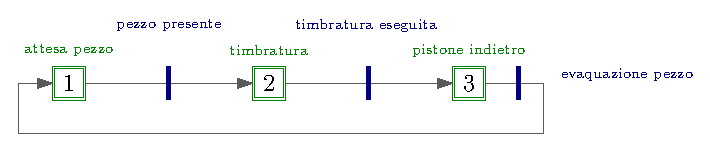
\includegraphics[width=0.7\textwidth ]{images/timbratrice.eps}
\end{center}
\flowerLine 
\section{Analisi dei Sistemi di Produzione}
Si considerino i sistemi di produzione manifatturiera, quindi, discreti. Essi possono seguire diverse strutture, 
fra le più importanti vi sono\begin{itemize}
    \item \textbf{linea di trasferta } : La produzione avviene secondo una specifica sequenza, rigida e non 
    flessibile. Un esempio tipico è la classica catena di montaggio introdotta da Ford. 
    \item \textbf{flow shop} : Vi sono diversi macchinari, e più flussi di produzione che si 
    alternano i macchinari diversi. 
    \item \textbf{job shop} : Ci sono differenti percorsi, intrecciati e complessi fra i diversi macchinari 
    e reparti dell'impianto di produzione. 
    \item  \textbf{celle di produzione} : Le singole celle contengono più macchinari, ed ognuna di queste 
    si occupa della produzione (dall'inizio alla fine) di un singolo prodotto, mantenendola concentrata 
    nella celle, senza che essa sia dislocata nell'impianto. 
    \item \textbf{FMS} : Diversi flussi fra le varie celle.
\end{itemize}
Vanno considerati vari aspetti nell'analisi dei sistemi di produzione, come la trattazione dei tempi di 
attesa, il \textit{WIP - work in process}, è un termine utilizzato per indicare il numero di pezzi che vengono 
lavorati contemporaneamente.
\begin{figure}[h!]
    \centering
    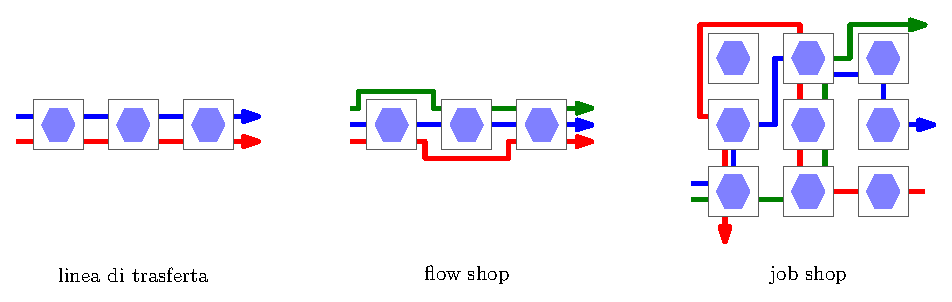
\includegraphics[width=0.8\textwidth ]{images/lineaFlowJob.eps}
    \caption{sistemi di produzione}
    \label{fig:sisprod}
\end{figure} 
\subsection{Linee di Trasferta}
Verrà trattata in questa sezione la modellizzazione delle linee di trasferta, e verranno analizzati 
alcuni parametri che le caratterizzano. Una linea di trasferta consiste in una serie di macchine o stazioni 
(macchinari adatti a più compiti) connessi sequenzialmente da un sistema di trasporto. La sequenza di produzione 
è rigida ed i pezzi vengono processati continuamente nel tempo senza interruzioni. Le linee possono essere 
sincrone e (i pezzi avanzano alla stessa velocità) oppure asincrone, tramite l'installazione di appositi 
buffer fra una macchina e l'altra.\begin{itemize}
    \item \textit{pro} : La produzione avviene per un singolo prodotto, risulta molto efficiente, il WIP è 
    ridotto ed il trasporto dei pezzi è semplice, dato che segue un unica direzione. I tempi di avvio sono brevi. 
    \item \textit{contro} : La produzione è poco flessibile ed è a rischio obsolescenza, il malfunzionamento 
    di una macchina può causare l'interruzione dell'intera linea (single point of failure).
\end{itemize}
\teo{(Legge di Little)} Data una linea di trasferta, ed i seguenti parametri \begin{itemize}
    \item $p$ : tasso di produzione misurato in pezzi per unità di tempo 
    \item $T_a$ : tempo necessario per l'attraversamento di una linea 
    \item $WIP$ il work in process,  il numero di pezzi che vengono 
    lavorati contemporaneamente
\end{itemize}
Vale la seguente relazione $$ WIP = p\cdot T_a$$
La legge si riferisce ad un sistema a regime permanente, quindi non considera l'avvio della linea, dato quindi 
un tasso $p$ fisso, per ridurre il $WIP$ è necessario ridurre il  tempo necessario 
per l'attraversamento della linea. 
\subsubsection{Esempio}
Verrà considerata una linea di trasferta composta da 3 macchine $M_1,M_2$ e $M_3$, i cui tempi di 
lavoro sono uguali e costanti $T_1=T_2=T_3=2$. Tale analisi è fatta a $WIP$ costante.
\begin{center}
    \includegraphics[width=0.5\textwidth ]{images/WIP1.eps}
\end{center}
In questo contesto, il WIP è 1, ciò significa che solamente un pezzo (indicato con una pallina verde) può 
occupare le 3 macchine contemporaneamente. Ogni 2 unità di tempo, il pezzo viene processato da una 
macchina all'altra, ci vogliono 6 unità di tempo per produrre un pezzo, $T_a=6$. 
$$T_a=6 \land WIP = 1 \implies p = \frac{1}{6} \text{ un pezzo ogni 6 unità di tempo}$$
\begin{center}
    \includegraphics[width=0.9\textwidth ]{images/WIP2.eps}
\end{center}
Si noti come nonostante il WIP aumenti, nel caso $WIP=4$ il tasso di produzione rimane invariato, 
risulta quindi fondamentale trovare il valore di WIP ottimale che minimizzi $T_a$ e 
massimizzi $p$. 
\begin{center}
    \begin{figure}[h!]
        \centering
        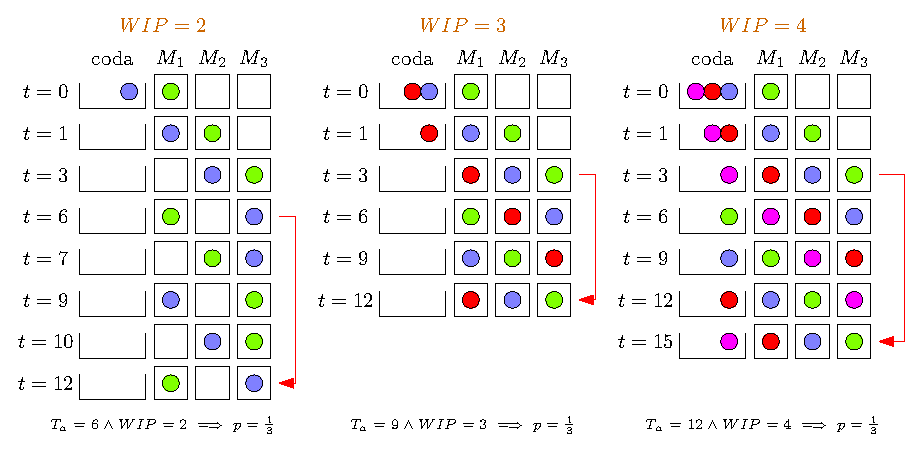
\includegraphics[width=0.9\textwidth ]{images/WIP3.eps}
        \caption{$ T_1 = 1\ \ \ \ \ T_2 = 2 \ \ \ \ \ T_3 = 3$}
        \label{fig:wip3}
    \end{figure}
\end{center}
L'esempio proposto in figura \ref{fig:wip3} è simile a quello precedente, ma in questo caso le macchine hanno tempi 
di lavoro differenti, precisamente, aumentano in ordine crescente. 
\begin{center}
    \begin{figure}[h!]
        \centering
        \includegraphics[width=0.9\textwidth ]{images/analisiWIP.eps}
        \caption{Analisi in funzione del $WIP$}
        \label{fig:wipAnalysis}
    \end{figure}
\end{center}
Con \textbf{Dimensionamento} e \textbf{Bilanciamento} di una linea di trasferta, si intende la ricerca del 
compromesso ideale fra l'aumento della produttività (utilizzo di più macchine) e la riduzione dei costi, 
a parità di tempo totale di lavorazione. Le curve in figura \ref{fig:carico}, descrivono l'allocazione delle 
lavorazioni (distribuzione del carico) in un numero fissato di $N$ stazioni/macchine.
\begin{figure}[h!]
    \centering
    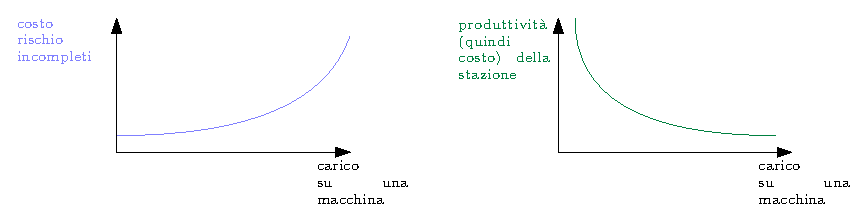
\includegraphics[width=0.9\textwidth ]{images/carico.eps}
    \caption{Analisi in funzione del carico su una singola macchina}
    \label{fig:carico}
\end{figure}
\begin{itemize}
    \item maggiore è il numero di stazioni utilizzate, minore sarà il carico medio delle
    stazioni e maggiore il costo unitario del singolo pezzo prodotto
    \item minore è il numero di stazioni utilizzate, maggiore sarà il carico medio delle
    stazioni e maggiore il costo del rischio di effettuare lavorazioni incomplete, 
    a causa della elevata saturazione nell'impiego dei macchinari della stazione
\end{itemize}
Il problema del bilanciamento di una linea di trasferta è NP-completo, per questo vengono utilizzate 
delle euristiche di soluzione, che garantiscono una soluzione prossima a quella ottimale. \acc 
\subsubsection{Modello del Problema del Dimensionamento}
Vi è una linea di trasferta con $n$ macchine/stazioni, ogni macchina $i$-esima, ha un carico di lavoro 
$C_i$ esepresso in unità di tempo. La linea deve soddisfare un certo tasso di produzione $p$ espresso in 
pezzi per unità di tempo. Il valore $CMT=\frac{1}{p}$ rappresenta il \textit{carico massimo teorico}, è 
chiaro che se una qualsiasi stazione ha un carico $C_i>CMT$, allora il tasso di produzione $p$ non è 
rispettato.\begin{quote}
    Un tasso $p=7200\frac{\text{pezzi}}{\text{mese}}=10\frac{\text{pezzi}}{\text{ora}}$ implica un 
    carico di lavoro massimo pari a $6$ minuti per pezzo. 
\end{quote}
Sarebbe ideale inoltre ridurre il numero delle macchine $n$, dato che più macchine, equivale a dire un costo 
di manutenzione maggiore. Nella linea di trasferta, le varie lavorazioni da eseguire possono avere 
delle \textit{dipendenze} (una lavorazione $i$ può essere eseguita esclusivamente dopo una lavorazione 
$j$), si possono quindi rappresentare tali dipendeze attraverso un grafo orientato. \acc 
Dato quindi un insieme di lavorazioni, si vuole trovare \begin{itemize}
    \item una sequenza di produzione in cui il carico di lavoro per ogni macchina sia minore del carico di lavoro massimo teorico (ammissibilità)
    \item tale sequenza, deve rispettare le dipendenze (ammissibilità)
    \item che minimizzi il numero $n$ di macchine/stazioni
\end{itemize}
\textbf{Esempio}\begin{center}
    \begin{tabular}{|c|c|c|c|c|c|c|c|c|c|c|c|c|c|c|}
        \hline
        Lavorazione                                                       & A  & B  & C  & D  & E  & F  & G                                                 & H                                                    & I  & J  & K  & L  & M  & N                                                    \\ \hline
        \begin{tabular}[c]{@{}c@{}}Tempo $T_i$ \\ in secondi\end{tabular} & 55 & 30 & 50 & 42 & 20 & 25 & 45                                                & 60                                                   & 36 & 42 & 30 & 40 & 36 & 40                                                   \\ \hline
        \begin{tabular}[c]{@{}c@{}}lavorazioni \\ necessarie\end{tabular} &    & A  & A  & A  &    &    & \begin{tabular}[c]{@{}c@{}}A, E,\\ F\end{tabular} & \begin{tabular}[c]{@{}c@{}}B, C,\\ D, G\end{tabular} & H  & H  & H  & J  & J  & \begin{tabular}[c]{@{}c@{}}I, K,\\ L, M\end{tabular} \\ \hline
        \end{tabular}\end{center}\begin{center}
        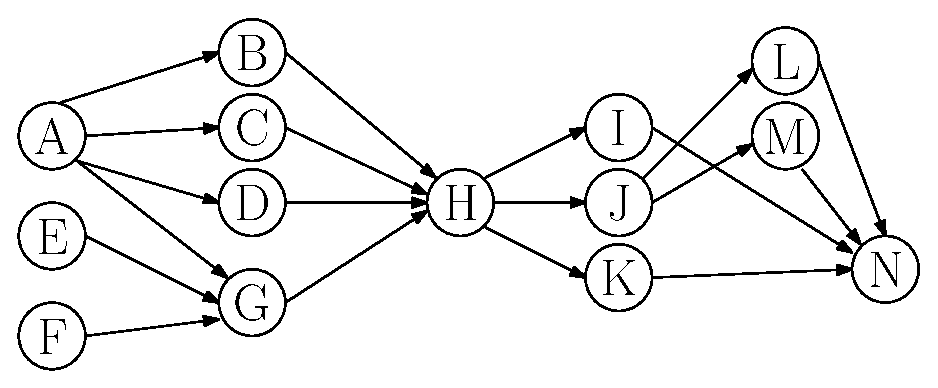
\includegraphics[width=0.7\textwidth ]{images/grafoDimensionamento.eps}
\end{center}
La specifica del tasso di produzione è $$p=300 \frac{pezzi}{7h}=\frac{300}{7}\frac{pezzi}{h}=
\frac{300}{3600*7}\frac{pezzi}{s}=\frac{1}{84}\frac{pezzi}{s}$$
Il carico massimo teorico è quindi $$CMT=p^{-1}=84\text{ secondi a pezzo }$$
Essendo il tempo totale per la lavorazione di un pezzo uguale a $551$ secondi, si ha che, al minimo, 
il numero di macchine presenti deve essere $n=\lceil\nicefrac{T_{tot}}{CMT}\rceil=\lceil\nicefrac{551}{84}\rceil=7$. Per trovare 
una sequenza ammissibile ed ottimale, sarebbe necessaria una procedura non polinomiale, esistono quindi degli algoritmi che 
forniscono una soluzione ammissibile (quando possibile) tramite delle euristiche.
\subsubsection{Ranked Positional Weight Technique}
L'algoritmo consiste nell'assegnare ad ogni lavorazione $i$ un peso $PW_i$, che consiste nel suo tempo necessario 
$T_i$ sommato ai tempi di tutte le lavorazioni che dipendono da esso, direttamente ed indirettamente. In seguito, si ordinano 
le lavorazioni in base a tali pesi, in ordine decrescente, nell'esempio precedente si ha \begin{center}
    \begin{tabular}{|c|c|c|c|c|c|c|c|c|c|c|c|c|c|c|}
        \hline
        Lavorazione & A                                                         & B                                                     & C                                                     & D                                                     & E                                                        & F                                                        & G                                                    & H      & I  & J                                                 & K  & L  & M  & N  \\ \hline
        $T_i$       & 55                                                        & 30                                                    & 50                                                    & 42                                                    & 20                                                       & 25                                                       & 45                                                   & 60     & 36 & 42                                                & 30 & 40 & 36 & 40 \\ \hline
        precedenti  & \begin{tabular}[c]{@{}c@{}}B, C, D\\ G..., N\end{tabular} & \begin{tabular}[c]{@{}c@{}}H, I\\ ..., N\end{tabular} & \begin{tabular}[c]{@{}c@{}}H, I\\ ..., N\end{tabular} & \begin{tabular}[c]{@{}c@{}}H, I\\ ..., N\end{tabular} & \begin{tabular}[c]{@{}c@{}}G, H ,\\ I,... N\end{tabular} & \begin{tabular}[c]{@{}c@{}}G, H ,\\ I,... N\end{tabular} & \begin{tabular}[c]{@{}c@{}}H, I\\ ...,N\end{tabular} & I...,N & N  & \begin{tabular}[c]{@{}c@{}}L, M,\\ N\end{tabular} & N  & N  & N  &    \\ \hline
        $PW_i$      & 506                                                       & 314                                                   & 334                                                   & 326                                                   & 349                                                      & 354                                                      & 329                                                  & 284    & 76 & 158                                               & 70 & 80 & 76 & 40 \\ \hline
        \end{tabular}
\end{center}
A tal punto si ordinano secondo $PW_i$ : $$A\rightarrow F \rightarrow  E \rightarrow  C \rightarrow  G 
\rightarrow D \rightarrow  B \rightarrow  H \rightarrow  J \rightarrow  L 
\rightarrow  I \rightarrow  M \rightarrow  K \rightarrow  N $$
Si iniziano poi a considerare le lavorazioni in quest'ordine una dopo l'altra, sommandone i tempi necessari fino 
a ché sono minori di $CMT$, ad esempio 
\begin{itemize}
    \item Considero A, che ha tempo di lavorazione $55$, lo assegno alla prima stazione. \\$\diamond $ Carico della stazione 1 : $C_1=55\le CMT$
    \item Considero F, che ha tempo di lavorazione $25$, lo assegno alla prima stazione. \\$\diamond $ Carico della stazione 1 : $C_1=80\le CMT$
    \item Considero E, che ha tempo di lavorazione $20$, non posso assegnarlo alla prima stazione, dato che il carico sarebbe 
    maggiore di $CMT=84$, quindi è necessaria una nuova stazione alla quale assegno E. \\$\diamond $ Carico della stazione 2 : $C_2=20\le CMT\le CMT$
    \item Considero C, che ha tempo di lavorazione $50$, lo assegno alla seconda stazione. \\$\diamond $ Carico della stazione 2 : $C_2=70\le CMT\le CMT$
    \item ...e così via
\end{itemize}
Al termine, si avrà la seguente assegnazione\begin{center}
    \includegraphics[width=0.6\textwidth ]{images/bilanciamentoLineaEs.eps}
\end{center}
Il termine $CMT-C_i$ è detto \textit{sbilanciamento}, lo sbilanciamento medio equivale  
alla somma degli sbilanciamenti diviso il numero di stazioni, in questo caso $\nicefrac{111}{8}=13.875$ secondi, 
si misura in percentuale rispetto il $CMT$, in questo caso, si ha uno sbilanciamento di circa $16.5\%$.
\begin{center}
    \includegraphics[width=1\textwidth ]{images/gantt.png}
\end{center}
\subsection{Flow Shop}
Un'altro tipo di struttura per un sistema industriale è il già citato flow shop, dove vi è la produzione 
di diversi prodotti, che devono seguire un determinato percorso fra le macchine presenti. Ogni prodotto 
deve vedere $m$ lavorazioni, e differenti prodotti, possono passare per la stessa macchina, ma 
necessitando di tempi differenti, quindi, sarà assegnato un tempo di lavorazione ad ogni 
coppia (lavorazione, prodotto). Il tempo totale di completamento $T_{max}$, detto \textbf{makespan}, è il 
valore da minimizzare, possono essere presenti dei buffer nella struttura.\acc Il problema si complica 
rispetto la linea di trasferta, in questo caso però, date per assunte delle condizioni, vi è una regola che permette 
di stabilire una sequenza ottimale.\acc 
\teo{(Regola di Jhonson)}
Assunzione : Ci sono esclusivamente 2 macchine/stazioni, denotate $M_1$ e $M_2$.\\
Sia $L=\{l_1,l_2\dots,l_n\}$ un insieme di lavorazioni, i  cui tempi per $M_1$ sono 
$\{t_{1_1},t_{2_1}\dots,t_{n_1}\}$, e i tempi per $M_1$ sono 
$\{t_{1_2},t_{2_2}\dots,t_{n_2}\}$. dove $\forall i, \ t_{i_1}>0\land t_{i_2}>0$. Nella \textbf{soluzione ottimale}, 
la lavorazione $l_i$ precede la lavorazione $l_j$ se e solo se 
$$ \min(t_{i_1},t_{j_2})<\min(t_{j_1},t_{i_2})$$
Tale teorema fornisce una procedura per trovare una soluzione ottimale, i passi sono i seguenti \begin{enumerate}
    \item si costruisce $S1=\{l_i\in L \ | \ t_{i_1}<t_{i_2}\}$
    \item si costruisce $S2=S1^C=\{l_i\in L \ | \ l_i\notin S1\}$
    \item Vengono schedulate le lavorazioni secondo la regola\begin{itemize}
        \item prima si eseguono tutte le lavorazioni di $S1$ in ordine crescente secondo $t_{i_1}$
        \item poi si eseguono tutte le lavorazioni di $S2$ in ordine decrescente secondo $t_{i_2}$
    \end{itemize}
\end{enumerate}
\subsubsection{Esempio di Applicazione per 2 Macchine}
Si hanno le seguenti lavorazioni \begin{center}
    \begin{tabular}{|c|c|c|c|c|c|c|}
        \hline
        Lavorazione & A & B & C & D  & E  & $T_{tot}$ \\ \hline
        $t_{i_1}$   & 5 & 3 & 8 & 10 & 7  & 33        \\ \hline
        $t_{i_2}$   & 2 & 6 & 4 & 7  & 12 & 31        \\ \hline
        \end{tabular}
\end{center}
Si costruiscono i due insiemi\begin{itemize}
    \item $S1=\{B, E\}$
    \item $S2=\{A, C, D\}$
\end{itemize}
Si ordinano secondo i criteri della procedura ottenendo la sequenza $$ S^* = 
B\rightarrow E\rightarrow D \rightarrow C \rightarrow A$$\begin{center}
    \includegraphics[width=0.8\textwidth ]{images/jhonson.eps}
\end{center}
Gli intervalli rossi nella linea del tempo rappresentano il \textit{tempo sprecato},
all'istante $t=20$, la lavorazione D termina su $M_1$, ed è pronta ad essere schedulata 
su $M_2$, ma quest'ultima è ancora impegnata nella lavorazione di E, per questo il prodotto 
che ha appena terminato D dovrà attendere, sarà quindi necessaria la presenza di un buffer. Situazione analoga 
per la lavorazione C nell'istante 28. \acc 
Non ci sono attese sulla macchina 1, le attese sulla macchina 2 sono inevitabili, ma tale procedura 
le minimizza. La macchina 1 è costantemente carica, si dice che $T_{idle,1}=0$ (non ci sono tempi di attesa). 
Differente è la situazione per la macchina 2 : $T_{idle,2}=4$. Il tempo di lavorazione totale è $T_{max}=35$.
\subsubsection{Generalizzazione con 3 Macchine}
Sotto ulteriori ipotesi, è possibile trovare una soluzione ottimale anche in un contesto con 3 macchine/stazioni $M_1,M_2,M_3$, 
con relativi tempi di lavorazione $t_{i_1},t_{i_2},t_{i_3}$ con $i\in\{1,2\dots ,n\}$ dove $n=$numero 
lavorazioni. Per poter 
trovare tale soluzione, è necessario che venga soddisfatta la seguente condizione 
$$ \max_{i\in\{1,2\dots ,n\}}(t_{i_2})\le \min_{i\in\{1,2\dots ,n\}}(t_{i_1}) \ \lor  
\max_{i\in\{1,2\dots ,n\}}(t_{i_2}) \le \min_{i\in\{1,2\dots ,n\}}(t_{i_3}) $$
Se tale condizioni è avverata, è possibile considerare una struttura flow shop a due macchine, precisamente $M'_1,M'_2$, con le 
medesime lavorazioni, la cua soluzione è identica alla soluzione del sistema originale con 3 macchine.\acc 
Nel nuovo sistema, i nuovi tempi di lavorazione $t'_{i_1},t'_{i_2}$ vanno definiti come segue \begin{itemize}
    \item $t'_{i_1}=t_{i_1}+t_{i_2}$
    \item $t'_{i_2}=t_{i_2}+t_{i_3}$
\end{itemize}
\subsubsection{Esempio di Applicazione per 3 Macchine}
Si hanno le seguenti lavorazioni \begin{center}
    \begin{tabular}{|c|c|c|c|c|}
        \hline
        Lavorazione & A & B & C & D \\ \hline
        $t_{i_1}$   & 4 & 1 & 5 & 2 \\ \hline
        $t_{i_2}$   & 3 & 2 & 3 & 3 \\ \hline
        $t_{i_3}$   & 3 & 4 & 5 & 3 \\ \hline
        \end{tabular}
\end{center}
La condizione $\max_{i\in\{1,2\dots ,n\}}(t_{i_2}) \le \min_{i\in\{1,2\dots ,n\}}(t_{i_3}) $ è soddisfatta, 
quindi posso ridurre il sistema ad uno equivalente \begin{center}
    \begin{tabular}{|c|c|c|c|c|}
        \hline
        Lavorazione & A & B & C & D \\ \hline
        $t_{i'_1}$   & 7 & 3 & 8 & 5 \\ \hline
        $t_{i'_2}$   & 6 & 6 & 8 & 7 \\ \hline
        \end{tabular}
\end{center}
Si applica la regola di Jhonson, trovando la sequenza $S^*=B\rightarrow D\rightarrow C\rightarrow A$, che verrà 
applicata al sistema originale con 3 macchine.\begin{center}
    \includegraphics[width=0.9\textwidth ]{images/jhonson2.eps}
\end{center}
Un altra struttura è la \textbf{produzione per reparti}, già accennata con il nome di \textbf{job shop},
in cui l'impianto è suddiviso in reparti contenenti stazioni, ed i vari prodotti devono essere passati fra i 
reparti attraverso sistemi di trasporto che seguono un percorso 
prefissato, è quindi necessario considerare il routing dei prodotti fra i reparti. Il modello job shop è caratterizzato 
da \begin{itemize}
    \item vaste categorie di prodotti, che subiscono lavorazioni con sequenze differenti 
    \item operazioni non ripetitive ed alta flessibilità 
    \item un maggiore work in process, i flussi lavorativi sono intricati 
    \item elevati tempi di attraversamento, e qualità dei prodotti non sempre omogenea
\end{itemize}
Quando è possibile individuare famiglie di prodotti simili con cicli di lavorazione omogenei si identificano delle 
celle contenenti gruppi di macchine adatti a tale famiglia di prodotti, tale \textbf{produzione per celle} semplifica 
i flussi di produzione, il trasporto e la gestione, le varie celle sono indipendenti fra loro.\acc
\begin{figure}[h!]
    \centering
    \includegraphics[width=0.65\textwidth ]{images/celleReparti.png}
    \caption{job shop e celle di produzione}
\end{figure}
Quando si implementa il trasporto automatico ed un controllo tramite calcolatore nelle celle di produzione si 
parla di \textbf{Flexible Manufacturing/Assembly Systems (FMS/FAS)}, sono sistemi dotati di elevata 
 flessibilità riguardo alle diverse sequenza delle lavorazioni 
 e/o all'assegnamento di operazioni alle risorse. Sono caratterizzati da \begin{itemize}
    \item diversi prodotti 
    \item lavorazioni eseguite su più macchine 
    \item assegnazione delle risorse tramite routing dei flussi 
    \item problemi di sequenziamento locale dell'impiego delle risorse 
    \item alto grado di automazione
 \end{itemize}
È possibile individuare tre tipi di automazione industriale\begin{itemize}
    \item \textit{Automazione rigida} : La sequenza delle operazioni è fissata, sono sistemi poco 
     flessibili (come le linee di trasferta) destinati a grandi produzioni con poca varietà di prodotto.
    \item \textit{Automazione programmabile} : Si può cambiare la configurazione del flusso di produzione in modo 
    da variare il prodotto, tipico delle industrie con produzione discreta a lotti. Vi è un tempo di attesa 
    fra un lotto ed un altro per la riconfigurazione del flusso.
    \item \textit{Automazione flessibile} : estensione dell'automazione programmabile in 
    cui è possibile diversificare la produzione senza avere tempi morti di 
    conversione dell'impianto,  i macchinari utilizzati sono caratterizzati sono altamente configurabili.
\end{itemize}
In generale, per i sistemi di automazione, esiste una correlazione qualitativa fra la quantità di prodotto fabbricata, ed il 
numero di prodotti distinti.\begin{center}
    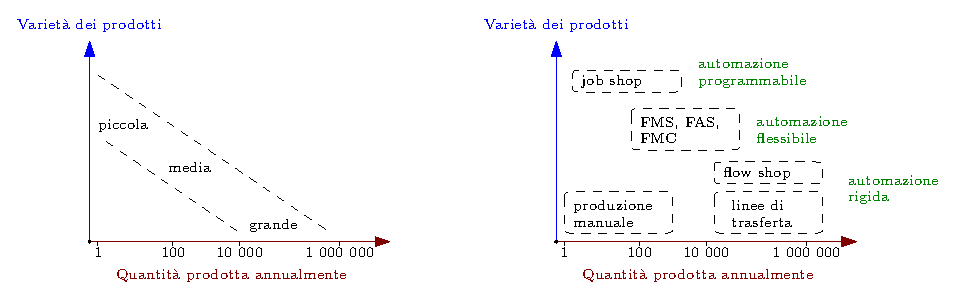
\includegraphics[width=1\textwidth ]{images/quantitVarieta.eps}
\end{center}\flowerLine 
\section{Sistema di Supporto}
Un sistema di supporto consiste in un insieme di attività legate all'impiano di produzione, in particolare\begin{itemize}
    \item attività di business, quali gestione degli ordini, marketing del prodotto e considerazioni economiche 
    \item progettazione del prodotto sulla base delle esigenze del mercato 
    \item pianificazione ("planning") della produzione, definizione della sequenza di lavorazione, politiche 
    di stoccaggio e rifornimento 
    \item controllo delle attività (gestione e supervisione)
\end{itemize}
Tali attività si re-iterano in un ciclo di produzione, cosiddetto "agile".
\begin{center}
    \includegraphics[width=0.3\textwidth ]{images/sistSupp.pdf}
\end{center}
In supporto delle attività di business vi sono \begin{itemize}
    \item \textbf{Enterprise Resource Planning (ERP)} : Un insieme di software volti all'automazione 
    dell'amministrazione, della logistica, della produzione e delle risorse umane. 
    \item \textbf{Decision Support System (DSS)} : Sistemi che hanno lo scopo, dato un insieme di dati 
    e dei vincoli da rispettare, di migliorare il processo decisionale nell'impianto.
\end{itemize}
Inoltre le macchine sul campo vengono supportate da sensori che hanno lo scopo di raccogliere dati ed informazioni 
in maniera massiva, in modo da poter essere utilizzati per i modelli di intelligenza artificiale e machine learning, 
sfruttando appunto,  tali dati per effettuare previsioni con maggiore precisione.
\acc In supporto alle attività di progettazione vi sono \begin{itemize}
    \item \textbf{Computer Aided Design (CAD)} : Un insieme di strumenti informatici utili nella progettazione. 
    \item \textbf{Computer Aided Engineering (CAE)} : Un insieme di strumenti informatici utili nella verifica 
    delle funzionalità tramite simulazioni e modelli matematici.
    \item \textbf{Computer Aided Manufacturing (CAM)} : Un insieme di software utili nell'automatizzazione ed 
    organizzazione delle sequenze di operazioni nella produzione.  
    \item \textbf{Computer Aided Process Planning (CAPP)} : software che 
    permette di automatizzare/ottimizzare il planning della produzione
\end{itemize}
È possibile utilizzare un modello CAD per ottenere un programma da eseguire su una CNC (macchina a controllo numerico)\begin{itemize}
    \item Caricamento di un modello CAD 
    \item Impostazione del sistema di coordinate 
    \item Impostazione di parametri 
    \item Generazione delle istruzioni per la macchina in questione 
    \item Invio dei dati al controllo numerico
\end{itemize}
\flowerLine 
\section{La Piramide CIM}
Quello della piramide CIM è un modello teorico che descrive la struttura di un processo produttivo, integrata 
con i sistemi di automazione ed i sistemi informatici gestionali, tale modello propone diversi vantaggi\begin{itemize}
    \item miglioramento della qualità di produzione 
    \item tempi e costi ridotti 
    \item aumento della flessibilità 
    \item diminuzione degli scarti e manutenzione predittiva 
    \item fondamentale per conformarsi a leggi e regolamenti sulla 
    sicurezza del processo produttivo, sulla qualità del prodotto e sulla riduzione dell'impatto ambientale
\end{itemize}
Il modello CIM è gerarchico e suddivide il processo di produzione su vari livelli, i cui elementi comunicano 
orizzontalmente con quelli adiacenti. Ogni livello assume che l'automazione nel livello inferiore sia 
ideale, nessun livello è privilegiato rispetto ad un altro.\begin{center}
    \includegraphics[width=0.6\textwidth ]{images/cim.pdf}
\end{center}
Dai livelli superiori le informazioni sono più elaborate e di minore quantità, ed i comandi vengono dati con minore 
frequenza, nei livelli inferiori, ci sono 
più informazioni, ma sono semplici, ed i comandi vengono dati con maggiore 
frequenza. La comunicazione verticala è privilegiata, se più dispositivi di campo devono 
comunicare, devono farlo attraverso il sistema di controllo della macchina di cui fanno parte. \acc 
Al livello di macchina e campo il controllo può essere sia \textit{logico} che \textit{diretto} (real time), 
attuato da microprocessori, con il salire dei livelli nella piramide il controllo assume sempre più un carattere 
logico, dettato da eventi.
\subsection{Livelli della Piramide}
\subsubsection{Livello di Campo}
Tale livello contiene dispositivi quali sensori ed attuatori, in generale,  i componenti hardware che 
eseguono le attività di produzione e controllo. Tali dispositivi interfacciano il livello superiore al livello 
fisico tramite segnali di ingresso ed uscita, possono inoltre comunicare informazioni sul proprio 
stato (auto diagnosi), oltre a ciò, sono generalmente semplici.\acc 
Sono raggruppati in semplici sistemi di controllo e i livelli superiori li assumono come dispositivi 
ideali, sono attrezzati di apposito hardware di controllo, quali sistemi digitali a microprocessori/sistemi 
embedded.
\subsubsection{Livello di Macchina}
Una macchina raggruppa più dispositvi di campo volti al fornire una determinata funzionalità. Ad esempio, 
diversi motori elettrici (dispositivi di campo) possono costituire un braccio robotico (macchina) volto allo 
spostamento di oggetti.\acc 
Tali componenti vengono controllati tramite dei controllori logici programmabili (PLC), tramite la regolazione 
di variabili analogiche e la realizzazione di sequenze di operazioni.\begin{quote}
    \color{gray}
    esempio: a livello di campo si controllano le posizioni dei singoli giunti; a livello di macchina 
viene pianificato il movimento del robot nello spazio operativo e la sequenza delle azioni che 
deve effettuare
\color{black}\end{quote}
\subsubsection{Livello di Cella}
Diverse macchine vengono ragruppate insieme formando delle celle di produzione, atte a produrre prodotti, anche 
diversi ma tecnologicamente affini, le macchine sono interconnesse fisicamente da un sistema locale di trasporto 
e stoccaggio. Nonostante il vincolo real time sia presente, il livello di controllo è quasi 
esclusivamente logico, e coordinano le macchine della cella. 
\subsubsection{Livello di Stabilimento}
Racchiude più celle e linee produttive di un impianto industriale, riceve istruzioni dal livello gestionale e le 
attua sotto forma di piani operativi per la produzione. I sistemi di controllo a tale livello sono denominati 
\textit{SCADA (Supervisory Control And Data Acquisition)}, tipicamente implementati in workstation. Sono sistemi di 
controllo che dispongono di\begin{itemize}
    \item Un interfaccia con l'operatore, assente nei microcontrollori e nei PLC 
    \item Gestione di allarmi e ricette 
    \item Programmazione dei lavori e basi di dati del processo produttivo 
    \item Controllo statistico e supporto alla manutenzione, potendo fare previsioni e rapporti
\end{itemize}
\begin{figure}[h!]
    \centering
    \includegraphics[width=0.65\textwidth ]{images/centrale (2).png}
    \caption{sala di controllo di una centrale elettrica}
\end{figure}
\subsubsection{Livello di Azienda}
Si occupa dei processi gestionali, il sistema non è di controllo ma \textit{decisionale}, costituito da un 
infrastruttura software connessa al mainframe aziendale, non esistono vincoli di tipo temporale.\acc 
Esiste uno standard (ANSI/ISA-S88.01-1995) che normalizza lo schema generale di controllo su 3 livelli gerarchici.
\begin{figure}[h!]
    \centering
    \includegraphics[width=0.7\textwidth ]{images/standardControlModel.pdf}
    \caption{modello delle attività di controllo}
\end{figure}
\begin{itemize}
    \item \textbf{controllo di campo} : controllo che agisce sui dispositivi di campo, in particolare, 
    su variabili continue, ed è impelentato su dispositivi dedicati. Le informazioni sono semplici 
    e trasmesse ad alta frequenza. 
    \item \textbf{controllo di procedure} : riguarda il controllo dei livelli di macchina e cella della 
    piramide, riguarda gruppi strutturati di componenti di campo, a tale livello vengono svolte funzioni di 
    auto-diagnostica, è implementato su schede dedicate o anche su pc industriali. Prevede 
    algoritmi più complessi di quelli del controllo di campo. Il controllo è \begin{itemize}
        \item \textit{diretto} : riguarda il controllo di 
        gruppi di variabili continue o funzioni più avanzate 
        \item \textit{logico} : coordinamento dei sistemi di campo sulla base della lista 
        di operazioni sequenziali
    \end{itemize}
    \item \textbf{controllo di coordinamento} : si pone al livello dello stabilimento ed opera su dati 
    strutturati a bassa frequenza, riguarda il coordinamento e la gestione delle varie celle di produzione, vincoli 
    temporali molto laschi.
\end{itemize}
\begin{center}
        \includegraphics[width=0.7\textwidth ]{images/cim2.pdf}
\end{center}
Lo standard definisce anche un diagramma logico delle transizioni tra stati di un processo. Si noti come 
i due stati \textit{Held} e  \textit{Paused} sono differenti: \begin{itemize}
    \item \textit{Paused} : è scaturita da un operatore esterno (esempio : causa operazioni di verifica) 
    \item \textit{Held} : il processo è in attesa di un evento e viene bloccato
\end{itemize}
\begin{center}
    \includegraphics[width=0.7\textwidth ]{images/statiProcesso.pdf}
\end{center}
\subsection{Auto-diagnostica}
I sistemi di controllo devono avere la possibilità di generare segnali ausiliari che danno allarme di eventuali guasti 
nei dispositivi soggetti ad usura. Occorre individuare dei segnali dal dispositivo che possono essere 
valutati secondo appropriati modelli matematici. \acc 
Con \textit{signature}, si definisce una firma del guasto, ossia una sua manifestazione sottoforma di segnale, un esempio 
può essere la misura tramite un accelerometro di vibrazioni in un sistema meccanico. Si sviluppano algoritmi atti 
all'analisi dei segnali (basati ad esempio sulla trasformata di Fourier).\acc 
Definiamo \textit{fault} i guasti, e li denotiamo $f$, su di essi si formulano\begin{itemize}
    \item \textit{fault detection} : rilevamento dei guasti sul sistema fisico o software 
    \item \textit{fault isolation} : classificazione del guasto, e distinzione di esso rispetto ad altri 
    \item \textit{fault identification} : determinazione del profilo temporale del guasto $f$ 
    \item \textit{fault accomodation} : riconfigurazione a seguito del guasto, coinvolge modifiche hardware o software
\end{itemize}
\subsubsection{Rilevazione ed Isolazione }
Quando un sistema dinamico è soggetto ad un possibile guasto, si definisce un sistema ausiliario detto 
\textbf{generatore di residuo}, il cui segnale in uscita dipenderà dalla presenza di un particolare guasto 
$f$. \begin{quote}
    Un residuo $r$ dipende da un guasto $f$
\end{quote}
Nel caso in cui possono esserci più guasti, si definisce un vettore $\bar r$ di residui, in cui $r_i$ dipende 
da $f_i$. Tipicamente il residuo riproduce approssimatamente l'evoluzione temporale del guasto. Con FDI si intende l'operazione 
di "Fault Detection Isolation", queste ultime due possono avvenire in contemporanea, vi sono differenti modelli proposti\begin{itemize}
    \item \textit{model-based} : si definisce un sistema dinamico che rappresenta il guasto (generatore di residuo)
    \item \textit{signal-based} : si utilizzano esclusivamente i segnali provenienti da misure del sistema, la loro 
    elaborazione può far luce su eventuali guasti 
    \item \textit{ibrido} : si combinano entrambe le tecniche
\end{itemize}
\subsubsection{Esempio di Residuo}
Vi è un processo (soggetto a guasto) modellato dal seguente sistema dinamico$$\begin{cases}
    \dot{x}=ax+bu+ef\\y=cx
\end{cases} $$
Dove $f$ è il generico fault. Il residuo $r$ viene implementato come osservatore di un disturbo, o di un 
segnale non noto (che in questo caso è $f$). 
$$ r(t)=\frac{k}{e}\Big[
\frac{y(t)}{c}-\int_0^t[ax(\tau)+bu(\tau)+er(\tau)d\tau]\Big] \ \  \text{ con }\ \ \begin{matrix}
    k>0\\ r(0)=0
\end{matrix}    
$$
L'evoluzione nel tempo del residuo è data da 
\begin{eqnarray}
    \dot{r}=\frac{k}{e}\Big[ \frac{\dot{y}}{c}-[ax+bu+er] \Big] = \\
    \frac{k}{e}\Big[ \frac{c[ax+bu+ef]}{c}-[ax+bu+er] \Big] = \\
    \frac{k}{e}e[f-r] = k[f-r]
\end{eqnarray}
Si ha quindi l'equazione lineare del primo ordine 
$$ kr+\dot{r}-kf=0$$
Si porta nel dominio di Laplace 
$$\mathcal{L}[kr+\dot{r}-kf](s)= $$ $$ 
k\mathcal{L}[r](s)+
\mathcal{L}[\dot{r}](s)-
k\mathcal{L}[f](s) = 
$$$$ 
k\mathcal{L}[r](s)+
s\mathcal{L}[r](s)-r(0)-
k\mathcal{L}[f](s) = 
$$
Si ricordi come $r(0)=0$. Denoto $\mathcal{L}[f]=F$ e $\mathcal{L}[r]=R$
$$ 
kR(s)+sR(s)-kF(s)=0\implies 
$$ $$ 
R(s)[k+s]=kF(s)
$$ 
$$
R(s)=\frac{kF(s)}{k+s} \implies 
$$ 
$$ \frac{R(s)}{F(s)}=\frac{k}{k+s}=\frac{1}{1+\frac{1}{k}s} $$
Nel caso il guasto fosse costante $f(t)=f_0$, nel dominio del tempo si avrebbe 
$$ r(t)=f_0[1-e^{-kt}]$$
\subsection{Architetture per il Controllo}
Il controllo è gestito da dispositivi elettronici ed informatici, è possibile individuare 3 tipi di 
sistemi\begin{itemize}
    \item \textbf{controllori embedded} - per il controllo di campo 
    \item \textbf{architettura a bus} - per il controllo di procedure 
    \item \textbf{PC-based}
\end{itemize}
\subsubsection{Sistemi Embedded}
Tali sistemi di controllo sono "fusi" alle funzionalità del dispositivo, e sono adoperati per un unico, specifico e 
predeterminato compito. Sono piattaforme hardware create "ad hoc", e la loro progettazione dipende dalla conoscenza dei 
compiti che dovranno svolgere. La realizzazione può avvenire in due modi \begin{itemize}
    \item singolo chip integrato (microcontrollori)
    \item singola scheda (DSP o FPGA)
\end{itemize}
L'hardware è semplice, vi è una CPU per gli algoritmi, una memoria per i dati ed i programmi e dei circuiti per 
gestire input ed output (analogici o digitali, con eventuali convertitori). Hanno un software integrato molto 
semplice ed è orientato all'automazione, vi è una gestione a basso livello delle risorse e delle comunicazioni.
\subsubsection{Microcontrollori}
I microcontrollori (a singolo chip) sono nati a seguito della miniaturizzazione dell'elettronica, sono 
utilizzati in una grandissima varietà di applicazioni e possono essere integrati con un sistema di sviluppo 
per la loro programmazione.\begin{figure}[h!]
    \centering
    \includegraphics[width=0.7\textwidth ]{images/auto.png}
    \caption{Sistemi di controllo embedded in automotive}
\end{figure}\acc
Caratteristiche ed impieghi : \begin{itemize}
    \item applicazioni semplici 
    \item basso consumo ed poco spazio occupato 
    \item numero limitato di segnali da gestire. Interfaccia utente assente 
    \item scarsa integrazione con dispositivi simili, difficile espansione
\end{itemize}
\subsubsection{Singola Scheda}
Prevedono più componenti standard integrati su una singola scheda, fra questi vi sono\begin{itemize}
    \item DSP (Digital Signal Processor) : processori atti al trattamento dei segnali ed esecuzione di funzioni su numeri interi o reali 
    \item FPGA (Field Programmable Gate Array) : circuiti integrati riconfigurabili dall’utente per realizzare 
    funzioni logiche complesse tramite blocchi logici e elementi di memoria
\end{itemize}
\begin{figure}[h!]
    \centering
    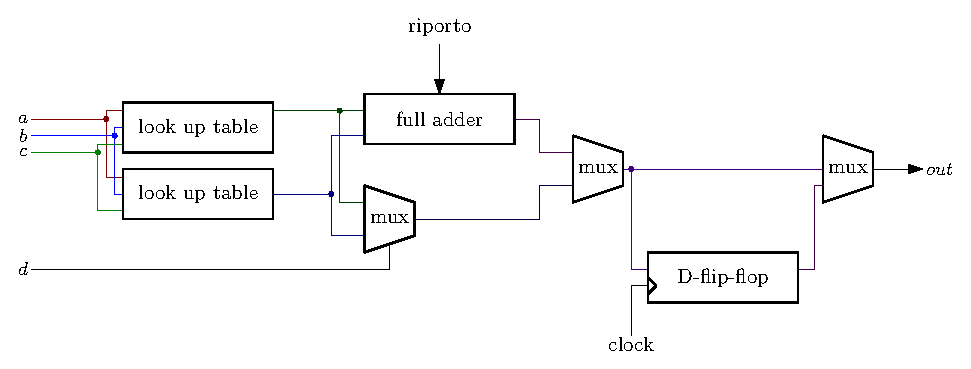
\includegraphics[width=0.7\textwidth ]{images/cellaLogica.eps}
    \caption{cella logica elementare in un FPGA}
\end{figure}
Rispetto i microcontrollori hanno una maggiore capacità di elaborazione e possono gestire un maggior numero 
di segnali.\acc 
Ricapitolando, i sistemi di controllo embedded prevedono i seguenti:\begin{itemize}
    \item \textbf{PRO}\begin{itemize}
        \item combinazione hardware/software specificamente studiata 
        \item ottimizzazione spaziale e di complessità
        \item minori ingombri, basso consumo 
        \item minori costi
    \end{itemize}
    \item \textbf{CONTRO}\begin{itemize}
        \item interfaccia uomo-macchina poco evoluta
        \item  gestione di un numero limitato di segnali in input/output 
        \item  costi di progettazione (hardware e software) non irrilevanti 
        \item poca flessibilità: modifiche ai compiti da svolgere possono 
        rendere necessaria la progettazione di un nuovo dispositivo 
    \end{itemize}
    Utili quando i compiti di controllo sono noti a priori.
\end{itemize}
\subsubsection{Architettura a Bus}
Con \textit{bus} si intende una linea elettrica che mette in comunicazione più dispositivi, vi è una scheda madre 
con un bus a cui si connettono più schede, in modo da rendere modulare il sistema. Un bus è composto da diverse 
linee\begin{itemize}
    \item linee dati 
    \item linee indirizzi 
    \item linee di alimentazione 
    \item linee per la comunicazione
\end{itemize}
\begin{figure}[h!]
    \centering
    \includegraphics[width=0.6\textwidth ]{images/bus.png}
    \caption{Modularità dell'architettura a bus}
\end{figure}
\begin{itemize}
    \item \textbf{PRO}\begin{itemize}
        \item flessibilità di progettazione 
        \item scelta dei moduli secondo le funzionalità da implementare
    \end{itemize}
    \item \textbf{CONTRO}\begin{itemize}
        \item Sistema Operativo più complesso
        \item  gestione dei moduli interconnessi e delle comunicazioni
        \item  vincoli real-time  
    \end{itemize}
\end{itemize}
\subsubsection{PC-Based}
Ultimamente, anche i comuni computer (corazzati per resistere alle condizioni 
sfavorevoli degli impiandi) sono adoperati  come sistemi di controllo, sono sistemi informatici con architettura  
a bus ed implementano una semplice interfaccia uomo macchina, e sono semplici da connettere alle reti informatiche.\acc 
Per far si che risultino efficaci come sistemi di controllo, esistono appositi sistemi operativi atti 
all'utilizzo real time (ad esempio, RTAI-Linux). Implementano 
moduli/schede per l'interconnessione con un elevato numero di 
segnali input/output, inoltre, esistono appositi protocolli per la comunicazione fra PC e PLC.
\flowerLine
\section{Industria 4.0}
La seconda rivoluzione industriale, agli inizi del $XX^\circ$ secolo ha introdotto la produzione di massa e la catena 
di montaggio classica (Ford), nei primi anni 70 l'avvento dei computer ed in particolare dei robot ha sondato la 
terza rivoluzione industriale, ad oggi vige l'industria 4.0 in cui le tecnologie ICT (Information and Communication Technology)
pervadono i processi produttivi. Anche la presenza di dispositivi intelligenti (IOT) capaci di fornire dati 
sulla rete tramite sensori e comunicare in tempo reale ha modificato il modo di produrre.\acc 
\textbf{Industria 4.0}:\begin{quote}
    \textit{“the comprehensive transformation of the whole sphere of
industrial production through the merging of digital technology and
the internet with conventional industry”} \\(Angela Merkel - Organization for
Economic Cooperation and Development, 19 Febbraio 2014)
\end{quote}
L'avvento di tali tecnologie ha portato un cambiamento industriale ma  anche sociale, e sono diventate necessarie 
diverse figure professionali che richiedono abilità trasversali per gestire le nuovo tecnologie. Definiamo le seguenti, 
\textbf{tecnologie abilitanti}\begin{itemize}
    \item \textit{Soluzioni manufatturiere avanzate} : utilizzo dei robot interconnessi e riprogrammabili 
    nell'automazione di attività precedentemente non automatizzabili.
    \item \textit{Additive manifacturing} : produzione per "addizione" di materiale, resa possibile dalle stampanti 
    3D connesse ai sistemi CAD. 
    \item \textit{Realtà aumentata} : l'uso della realtà aumentata e della realtà virtuale ha permesso la 
     simulazione di processi fisici a supporto dei processi produttivi. 
     \item \textit{Simulazione} : Simulazione in tempo reale del sistema di produzione in grado di 
        migliorare il processo decisionale e predittivo tramite l'uso dei digital twin.
    \item \textit{Integrazione orizzontale/verticale} : Integrazione di informazioni lungo la catena del valore, dal consumatore 
    al fornitore. 
    \item \textit{Internet industriale} : Comunicazione multidirezionale diffusa tra processi produttivi e prodotti. 
    \item \textit{Cloud} : Uso del cloud per la raccolta dei dati in maniera distribuita.  
    \item \textit{Sicurezza} : Metodologie di difesa alle minaccie informatiche alla quale sono soggetti i 
    sistemi aperti ed interconnessi.  
    \item \textit{Big data} : Uso dei modelli volti all'analisi statistica dalle grandi quantità di dati 
    disponibili allo scopo di estrarne informazioni. 
\end{itemize}
L'uso delle tecnologie abilitanti porta vari benefici\begin{itemize}
    \item Flessibilità nella produzione di piccoli lotti ai costi della grande scala 
    \item Maggiore velocità della progettazione e produzione dei prodotti 
    \item Maggiore produttività e riduzione dei tempi morti (tempi di setup, errori e fermi macchina)
    \item Migliore qualità del prodotto e riduzione degli scarti grazie a sensori che monitorano la produzione in tempo reale  
\end{itemize}
I sistemi ICT hanno permesso la creazione di modelli di business favoriti e definiti da 
apposite linee guida di sviluppo.\subsection{Tecnologie Abilitanti}
I \textbf{collaborative robots}, o più semplicemente \textit{cobots}, permettono la collaborazione 
fisica fra robot ed operatori rimuovendo le barriere dell'area di lavoro, questi ultimi entrano in contatto 
diretto, sono sensibili all'ambiente circostante grazie a sensori laser e sistemi di visione, ed appositi sistemi di controllo programmati 
per il riconoscimento e rilevamento di possibili urti con gli operatori. Presentano spesso strutture leggere e sono 
dotati di cedevolezza nei giunti, in grado di assorbire energia da urti esterni. Lo spazio di lavoro condiviso apre 
le possibilità a nuove applicazioni. \\\begin{figure}[h!]
    \centering
    \includegraphics[width=0.6\textwidth ]{images/cobot.png}
    \caption{Robot collaborativo}
\end{figure}\\
L'\textbf{additive manifacturing} permette la produzione di oggetti tridimensionali di varia forma a partire da 
un modello digitale CAD, la loro produzione richiede il materiale strettamente necessario per la stampa diminuendo i 
residui.\\\begin{figure}[h!]
    \centering
    \begin{tikzpicture}
        \pie{3.8/architettura, 4.5/altro, 17.3/veicoli, 12.3/aereospazio, 18.5/macchine industriali,
        6.4/uso militare, 18/elettronica, 
        13.7/apperecchiatura medica, 6.4/uso accademico}
    \end{tikzpicture}
    \caption{Uso della stampa 3D}
\end{figure}\\
I \textbf{digital twin} definiscono la programmazione e previsione dei sistemi tramite simulazioni digitali, utili durante la 
progettazione della linea di produzione, inoltre, in fase di esecuzione di essa è possibile eseguire in contemporanea il modello 
digitale in modo da supervisionare il processo.\acc 
Le tecniche di \textbf{machine learning} permettono il processamento di informazioni al fine di migliorare la qualità del 
prodotto grazie alla manutenzione predittiva.\acc 
L'\textbf{IOT} (Internet Of Things) riguarda i dispositivi capaci di rilevare e processare dati 
dal mondo fisico (temperatura,
illuminazione, umidità, ...) ha applicazioni di notevole impatto, ad esempio, in ambito medico, tali dispositivi 
condividono informazioni e comunicano con gli altri dispositivi e macchine connesse in rete.\\\begin{figure}[h!]
    \centering
    \includegraphics[width=0.6\textwidth ]{images/iot.jpg}
    \caption{Un'illustrazione di come questa rivoluzione 
    nella medicina apparirà in un tipico ospedale che fa uso di IOT}
\end{figure}\\
Le diverse tecnologie vengono incanalate in determinate linee guida di sviluppo, i sistemi distribuiti che permettono 
la circolazione rapida di informazioni sono combinati ad una centralizzazione della gestione di essi, garantendo la possibilità 
di controllare e monitorare in modo efficiente dati e risorse da e in qualsiasi parte dell'azienda.\acc Nonostante le 
macchine moderne siano indipendenti da un intervento continuo, devono essere supervisionate da un operatore umano, 
quest'ultimo deve avere la possibilità di intergarie con esse in maniere intuitiva, la branca che si occupa di rendere 
semplice tale operazione è denominata \textit{interazione uomo macchina}.
\subsection{Modelli di Business}
2 aspetti sono fondamentali nell'industria 4.0\begin{itemize}
    \item Qualità delle aziende migliorate grazie all'uso delle nuove tecnologie 
    \item Nuovi schemi di competizione del mercato basati sui nuovi modelli di business 
\end{itemize}
Tali modelli di business si sono sviluppati solo dopo l'avvento delle tecnologie abilitanti che li hanno resi 
realizzabili.\begin{itemize}
    \item \textbf{Centralità del cliente} : al centro della catena del valore dell'industria, c'è il cliente, il 
    consumatore, e le aziende puntano al soddisfare le richieste di quest'ultimo, talvolta anticipandone le necessità e le 
    richieste di servizio.
    \item \textbf{Economia circolare} : risponde alla necessità di passare ad un modello circolare di produzione, in 
    cui i prodotti ed i processi manifatturieri vanno improntati al riutilizzo.\begin{center}
        progetta $\longrightarrow$ usa $\longrightarrow$ ricicla $\longrightarrow$ riusa
    \end{center}
    Tale modello porta un risparmio dovuto alla riduzione degli scarti e ai minori costi di approvvigionamento, nonché 
    una notevole riduzione dell'impatto ambientale.
    \item \textbf{Strategie basate su ICT} : emergono nuove strategia di mercato che hanno lo scopo di portare il prodotto 
    più vicino al consumatore, le tecnologie alla base dell'industria 4.0 mettono a disposizione una grande mole di dati 
    utili al miglioramente dell'efficenza dell'azienda. \begin{itemize}
        \item negozi online 
        \item servizi ad abbonamento 
        \item affitto di infrastrutture informatiche 
    \end{itemize}
    \item \textbf{Economia della condivisione} : modelli di condivisione di beni e servizi tramite piattaforme digitali, come 
    i servizi di car sharing o bike sharing, irrealizzabili senza un infrastruttura informatica, che permette il monitoraggio 
    dello stato dei veicoli.
    \item \textbf{Economia del fare} : le stampanti 3D, grazie alla prototipazione rapida, hanno permesso l'insorgere di un "artigianato digitale" 
    autoprodotto a basso costo, con uso di materiali  plasmabili e anche di robot programmati.
\end{itemize}
\subsubsection{Cloud Automation}
I robot di servizio nei centri di \textit{Amazon} che si occupano dello stoccaggio 
dei prodotti funzionano grazie a degli algoritmi di instradamento che 
ne determinano i percorsi ottimali, tali algoritmi molto spesso risultano 
costosi da un punto di vista computazionale, de facto, i robot di questo tipo 
inviano i dati ad un server centralizzato che si occupa di eseguire gli algoritmi per 
poi restituire i risultati ai robot.\acc 
Un aspetto fondamentale dell'industria 4.0 è il processo di 
\textbf{trasformazione digitale} nelle aziende tramite l'inclusione delle 
tecnologie ICT, in particolare, sono identificati 6 passi 
fondamentali nella trasformazione, che incrementano il valore 
dell'azienda e del prodotto finale.
\\\begin{figure}[h!]
    \centering
    \includegraphics[width=1\textwidth ]{images/trasformazioneDigitale.png}
    \caption{i 6 passi della trasformazione digitale}
\end{figure}\\
 Ovviamente tale processo ha dei costi da sostenere, banalmente 
 l'implementazione di hardware e software, inoltre,è soggetto 
 ad errori che possono comportare rischi non di poco conto, i quali\begin{itemize}
    \item mancanza di una strategia chiara 
    \item mancanza di consenso ed impegno nella leadership
    \item concentrazione sulle tecnologie piuttosto che sulle persone 
    \item farsi guidare dalle tendenze senza avere una visione
    \item trascurare il contributo dei clienti
    \item voler organizzare il processo in autonomia 
    \item sottovalutare le competenze interne 
    \item non considerare la sicurezza dei dati 
    \item mancanza di flessibilità 
    \item carenza di comunicazione 
    \item sottovalutazione delle complessità
 \end{itemize}
La \textit{McKinsey} nel 2017 ha rilasciato un rapporto riguardante le attività lavorative ed il possibile 
grado di automatizzazione di queste, in particolare, si hanno i seguenti risultati, su un analisi che ha coinvolto 
circa 2000 attività lavorative relative a circa 800 occupazioni\begin{itemize}
    \item Storicamente l'automazione ha aumentato la produttività del (circa) $1\%$ all'anno
    \item Con le attuali tecnologie (in riferimento al 2017), è possibile automatizzare circa la metà delle 
    attività lavorative 
    \item Le attività che si prestano maggiormente ad essere automatizzate, son quelle che caratterizzano lavori 
    fisici, prevedibili e ripetitivi, che richiedono tipicamente un basse capacità cognitive. Costituiscono circa 
    il 51\% delle attività negli USA
    \item Le occupazioni le cui attività possono essere completamente automatizzate sono circa il 5\% 
    \item Nel 60\% delle occupazioni, circa il 30\% delle attività può essere atuomatizzato 
    \item Il lavoro umano affiancato ai robot è necessario a garantire la crescita del PIL
\end{itemize}\begin{center}
    \includegraphics[width=0.8\textwidth ]{images/attivitaAutomatizzabili.pdf}
\end{center}\begin{figure}[h!]
    \centering
    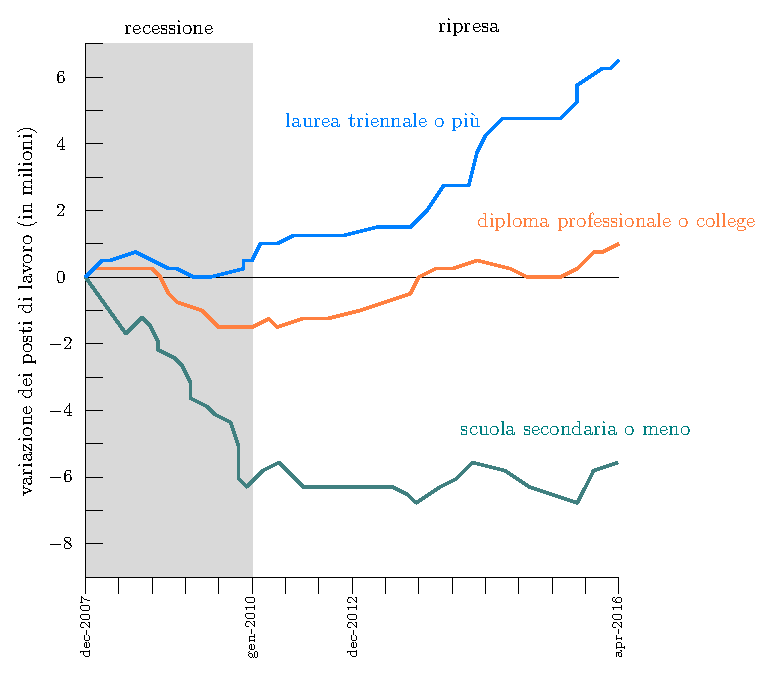
\includegraphics[width=0.6\textwidth ]{images/andamentoLavori.eps}
    \caption{Andamento dei posti di lavoro in base al livello di educazione}
\end{figure}
\subsection{Industria 5.0}
La commissione Europea ha trattato un rapporto sull'industria 5.0, che mira a sviluppare  il modello dell'industria 
4.0 verso un'industria europea sostenibile, resiliente e centrata sulla persona. Il progetto di 
ricerca \textit{Horizone Europe} punta ad investire sui progetti di ricerca che incorporino tali modelli, in Italia, 
il \textbf{PNNR} è un insieme di iniziative che puntano alla trasformazione dei sistemi di produzione, in particolare\begin{enumerate}
    \item digitalizzazione, innovazione, cultura 
    \item transazione al verde 
    \item infrastrutture per una mobilità sostenibile 
    \item istruzione e ricerca 
    \item coesione ed inclusione sociale 
    \item salute
\end{enumerate}
Come già accennato, le parole chiave dell'industria 5.0 sono le seguenti\begin{itemize}
    \item \textbf{resilienza} : gestire i cambiamenti desiderati e non (ad esempio, pandemie) con una 
    produzione  industriale
    dotata di supporti per le
    infrastrutture critiche e
    resistente a "interruzioni".
    \item \textbf{centralità della persona} : mettere l'essere umano al primo posto e chiedersi cosa 
    può fare la tecnologia per noi, e non cosa possiamo fare noi per la tecnologia, in particolare, adottarla 
    per adattare i processi produttivi alle necessità dei lavoratori.
    \item \textbf{sostenibilità} : economia circolare, riduzione dei rifiuti e dell'impatto ambientale, assicurare 
    i bisogni odierni senza mettere
    a repentaglio le future
    generazioni.
\end{itemize}



\chapter{Reti per l'Automazione}
Molti dei concetti trattati in questo capitolo, sono considerati più approfonditamente negli appunti del 
corso di 
\color{blue}\href{https://github.com/CasuFrost/University_notes/blob/main/Secondo%20Anno/Secondo%20Semestre/Reti%20di%20Elaboratori/Latex%20source%20file/Reti%20di%20Elaboratori.pdf}{Reti di Elaboratori}\color{black}.
\section{Sistemi di Comunicazione}
Le informazioni vengono condivise orizzontalmente e verticalmente 
fra i livelli della piramide CIM, in particolare\begin{itemize}
    \item si acquisiscono informazioni 
    \item si elaborano strategie 
    \item si attuano azioni correttive
\end{itemize}
I sistemi di comunicazione devono essere adeguati 
al garantire il flusso di informazioni fra i vari livelli della 
rete che differiscono nelle caratteristiche\begin{itemize}
    \item tipologie di dati differenti 
    \item differenti vincoli di comunicazione (ad es. il livello di campo 
    avrà dei vincoli real time)
\end{itemize}
È necessaria una standardizzazione dei protocolli di comunicazione digitale.
\begin{center}
    \includegraphics[width=0.8\textwidth ]{images/reti.png}
\end{center}
Gli elementi base di una rete sono \begin{itemize}
    \item Un mittente 
    \item Un destinatario 
    \item Un mezzo fisico sul quale viaggerà l'informazione 
\end{itemize}
I dati sono sul mezzo delle informazioni fisiche (luce, tensioni 
elettriche), i segnali possono essere analogici o digitali, 
in base alla definizione del protocollo. Il tipo di 
trasmissione può variare a seconda di diversi fattori, 
quali la \textbf{direzione}\begin{itemize}
    \item \textit{Simplex} : la trasmissione è unidirezionale 
    \item \textit{half duplex} : la trasmissione è bidirezionale ma 
    alternata, non si può trasmettere informazione in entrambe le direzioni 
    nello stesso momento
    \item \textit{full duplex} : bidirezionale simultanea 
\end{itemize}
il posizionamento dei bit\begin{itemize}
    \item \textit{parallela} : i bit di un byte vengono trasmessi 
    in parallelo su più canali, viene usata su distanze ridotte causa la 
    facile interferenza alla quale son soggetti.
    \item \textit{seriale} : il mezzo fisico è tipicamente 
    suddiviso in "invio","ricezione" e "massa", ed i bit di un byte 
    sono trasmessi in sequenza uno dopo l'altro. Quest'ultima può 
    a sua volta essere\begin{itemize}
        \item sincrona : i dati sono trasmessi continuamente insieme 
        ad un segnale di sincronizzazione 
        \item i dati sono trasmessi in modo irregolare a frequenza costante, 
        con bit di sincronizzazioni incapsulati nei dati 
    \end{itemize}
\end{itemize}
Le reti industriali prevedono solitamente una trasmissione digitale 
half duplex, seriale ed asincrona.\\\begin{figure}[h!]
    \centering
    \includegraphics[width=0.85\textwidth ]{images/protocolliReti.pdf}
    \caption{tipi di reti e protocolli industriali}
\end{figure}\\
Le \textit{Rete Enterprise} sono adottate per le informazioni gestionali e seguono il classico 
modello client-server, non hanno vincoli di real-time, più che la "robustezza" dell'informazione rispetto 
ai disturbi ambientali (che possono essere presenti in una cella), è importante 
la sicurezza e la riservatezza di esse. Tali reti seguono lo standard Ethernet, e sfruttano i 
protocolli di rete e di trasporto (ossia, IP e TCP) per garantire la ritrasmissione sicura dei dati 
in caso di perdite di pacchetti.\acc 
Le reti al livello di \textit{Controllo e Campo} invece gestiscono le informazioni nelle celle 
e fra le varie macchine, i dispositivi comunicanti spesso non sono standard, ma sono PLC, controllori embedded, 
e dispositivi di campo, quindi è importante che i protocolli in tale livello siano flessibili ed 
adattabili all'eterogeneità dei client.\acc  Qui i dati trasmessi hanno piccole dimensioni, ma la 
frequenza di trasmissione è alta, e deve soddisfare i vincoli real time, per questo Ethernet non è 
appropriato e si utilizzano soluzioni apposite. Essendo l'ambiente industriale "ostile", i mezzi di 
trasmissione devono essere robusti, i ritardi nella trasmissione nella struttura ad anello dei controllori 
possono causare un degrado nelle prestazioni non trascurabile, è più che mai necessario \textit{determinismo} nella 
trasmissione.
\flowerLine 
\section{Classificazione ed Architetture delle Reti}
Nel livello di campo, esistono due possibili architetture della rete da adottare che si 
differenziano nella topologia della rete ed altri fattori. In particolare\begin{itemize}
    \item \textbf{Architettura tradizionale} : Un architettura centralizzata in cui il controllore 
    prevede un collegamento punto-punto con ogni altri dispositivo di campo.\acc 
    \textit{Vantaggi}\begin{itemize}
        \item sistema affidabile e collaudato 
        \item disponibilità di tutte le tipologie di
        strumentazione sul mercato
    \end{itemize}
    \textit{Svantaggi}\begin{itemize}
        \item elevato numero di collegamenti 
        \item cablaggio costoso 
        \item lavoro di stesura e protezione dei fili critico
    \end{itemize}
    \item \textbf{Architettura a bus di campo (fieldbus)} : Un architettura che prevede la presenza di 
    un bus centrale (la cui comunicazione è digitale)
     alla quale ogni dispositivo si connette direttamente.\acc
     \textit{Vantaggi}\begin{itemize}
        \item installazione più economica 
        \item modularità : è facile aggiungere e rimuovere dispositivi 
        \item tolleranza ai guasti 
        \item condivisione delle risorse
    \end{itemize}
    \textit{Svantaggi}\begin{itemize}
        \item i dispositivi comunicano sullo stesso mezzo, è quindi necessario un protocollo di 
        accesso al mezzo 
        \item difficile da installare in aree pericolose
    \end{itemize}
\end{itemize}\begin{figure}[h!]
    \centering
    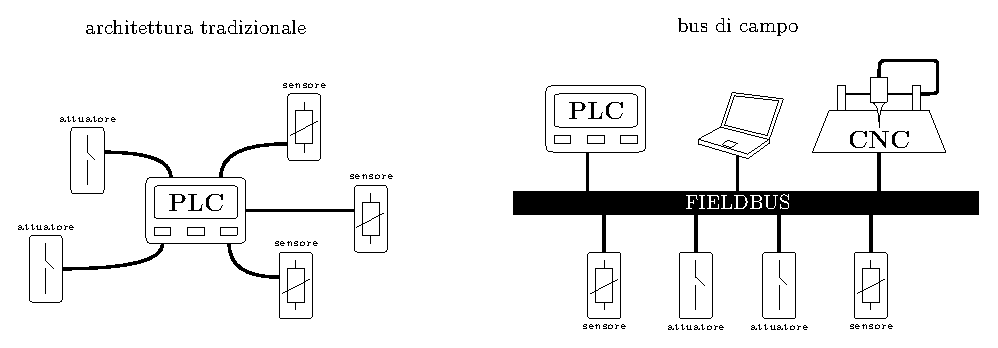
\includegraphics[width=0.85\textwidth ]{images/tradVSfieldbus.eps}
    \caption{soluzioni a livello di campo}
\end{figure}
\subsection{Tipologie di Reti}
Una rete può essere\begin{itemize}
    \item \textbf{broadcast} : vi è un unico canale di comunicazione condiviso da ogni macchina 
    sulla rete, i messaggi arrivano ad ogni nodo, i nodi scarteranno i messaggi di cui non sono 
    destinatari. Queste possono essere a loro volta\begin{itemize}
        \item \textit{reti a bus} : canale condiviso, in ogni istante un solo nodo può trasmettere 
        contemporaneamente, è necessario arbitraggio. 
        \item \textit{reti ad anello} : i pacchetti circolano in serie su un anello, necessario 
        arbitraggio per accessi simultanei
    \end{itemize}
    \begin{center}
        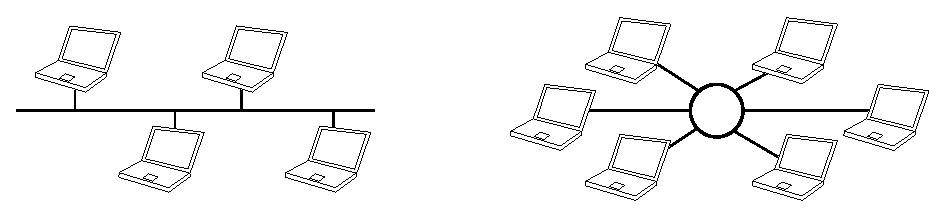
\includegraphics[width=0.85\textwidth ]{images/anelloEbus.eps}
    \end{center}
    \item \textbf{peer-to-peer} : per ogni coppia di nodi vi è una connessione dedicata, 
    se due macchine non sono connesse fisicamente, è necessario definire un cammino fra di esse tramite 
    appositi algoritmi di routing, 
    se più pacchetti relativi allo stesso messaggio seguono cammini diversi, è
    necessario gestire anche la sequenza con cui essi vengono ricevuti. Vengono applicate a reti di dimensioni maggiori, normalmente 
    più reti LAN sono connnesse in tal modo.\begin{center}
        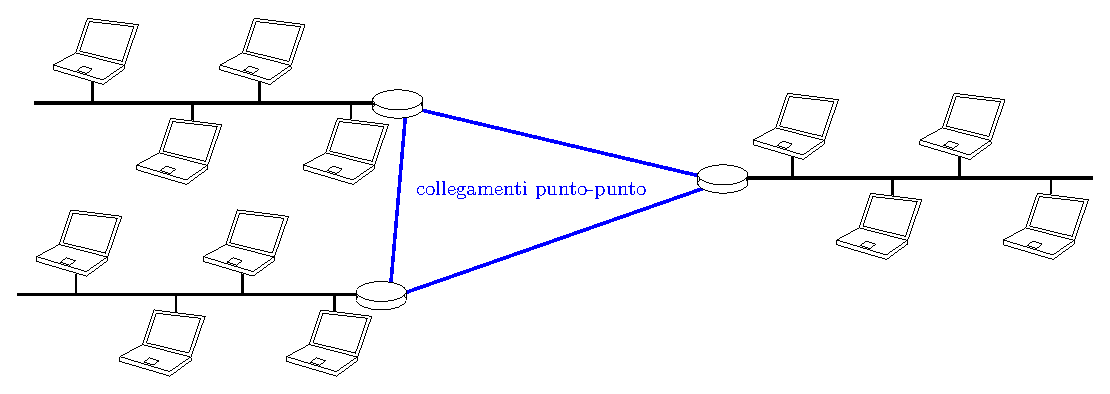
\includegraphics[width=0.85\textwidth ]{images/puntopunto.eps}
    \end{center}
    \item Nella maggioranza delle applicazioni più complesse, la soluzione più frequente 
    ricade in \textbf{reti ibride}.
\end{itemize}
Esiste una scala di classificazione delle reti :\begin{center}
    \begin{tabular}{|
            >{\columncolor[HTML]{EFEFEF}}c |
            >{\columncolor[HTML]{FFFFFF}}c |c|
            >{\columncolor[HTML]{FFFFFF}}c |}
        \hline
        \cellcolor[HTML]{9AFF99}{\color[HTML]{000000} Scala} & \cellcolor[HTML]{9AFF99}Tipo & \cellcolor[HTML]{9AFF99}Nome completo & \cellcolor[HTML]{9AFF99}Esempio \\ \hline
        Distanza ravvicinata                                 & PAN                          & Personal Area Network                 & Bluetooth                       \\ \hline
        Edificio                                             & LAN                          & Local Area Network                    & WiFi, Ethernet                  \\ \hline
        Città                                                & MAN                          & Metropolitan Area Network             & Cablata, DSL                    \\ \hline
        Paese                                                & WAN                          & Wide Area Network                     & Grandi ISP                      \\ \hline
        Pianeta                                              & Internet                     & La rete di tutte le reti              & L'Internet                      \\ \hline
    \end{tabular}
\end{center}
La \textbf{LAN} è la rete locale, come una rete domestica, è una rete privata ed ogni terminale connesso ad essa è identificato
da un indirizzo distinto dagli altri, può essere a \textit{cavo condiviso} oppure a \textit{commutazione} con uno switch.
In tale modello di cavo condiviso il pacchetto inviato ad un dispositivo viene ricevuto da tutti, solo il destinatario lo
elaborerà, tutti i restanti host lo ignoreranno.\acc
Quest'ultimo a commutazione è il più utilizzato tutt'oggi, ogni dispositivo è direttamente collegato allo switch, ed esso è
in grado di riconoscere gli host ed inviare i pacchetti esclusivamente al destinatario, riduce il traffico nella LAN.\acc
Le reti \textbf{WAN} sono reti geografiche, vengono interconnessi dispositivi di comunicazione, necessari a città, regioni o
perfino nazioni. I dispositivi in questione sono switch, router e modem, tale rete è gestita da un grande operatore/ente di
telecomunicazioni detto IPS (Internet Service Provider) che fornisce i servizi alle organizzazioni.\acc Una WAN può vedere i suoi
dispositivi di comunicazione connessi punto-punto, oppure a commutazione, con più punti di terminazione (usata nelle dorsali di
Internet), tutt'oggi è raro trovare LAN o WAN isolate, spesso sono connesse fra loro per formare una internetwork (internet), per
mettere in comunicazione due LAN in città differenti tramite una WAN.
\subsubsection{Dispositivi di Interconnessione}
Per il collegamento fra tratti di una stessa rete, oppure fra reti diverse, sono coinvolti vari dispositivi\begin{itemize}
    \item \textbf{repeater (ripetitore)} : amplifica e ricostituisce il segnale originale su segmenti analoghi della
    stessa rete [repeater RS485]
    \item   \textbf{hub (concentratore)} : estende una rete a stella, amplifica e ricostituisce lo stesso segnale su
    tutte le porte, non riduce le collisioni [Ethernet hub] 
    \item  \textbf{switch (interruttore)} : come un hub, ma su una singola porta per volta, può ridurre le
    collisioni [Ethernet switch]
    \item \textbf{transceiver (ricetrasmettitore)} : connette a una stessa rete segmenti di diversa tipologia
    [RS232/RS485 transceiver]
    \item \textbf{bridge (ponte)} : connette due reti che usano lo stesso protocollo ma che hanno layer
    differenti al livello inferiore [Modbus RS485 / Ethernet TCP-IP bridge]
    \item  \textbf{router (instradatore)} : connette due reti dello stesso tipo [Ethernet TCP-IP router] 
    \item \textbf{gateway (portale)} : connette due reti di tipo diverso [Ethernet / Modbus gateway] 
\end{itemize}
Nelle reti broadcast, l'accesso al canale può venire per vie di allocazione \begin{itemize}
    \item \textbf{statica} :  il tempo viene suddiviso in time slices (quanti) e ad ogni nodo 
    viene dedicato un intervallo periodico in cui può comunicare, nel caso non abbia nulla 
    da trasmettere, il canale resta inutilizzato (spreco di banda). 
    \item \textbf{dinamica} : Si suddivide in \begin{itemize}
        \item controllo centralizzato : un nodo \textit{master} determina il prossimo 
        dispositivo che potrà comunicare tramite strategie di polling. 
        \item controllo decentralizzato : ogni nodo decide autonomamente se trasmettere o no. 
        \item sistemi a collisione : i nodi possono trasmettere, se capita che due di essi 
        trasmettano contemporaneamente, vi sarà una \textit{collisione} che verrà 
        rilevata ed eventualmente risolta.
    \end{itemize}
\end{itemize}
\subsubsection{Architettura Software}
I 5 macro-livelli sulla quale si fonda la comunicazione sono i seguenti :
\begin{center}
    \includegraphics[width=1\textwidth ]{images/livelli.eps}
\end{center}
Sino ad ora i dati incapsulati che vengono comunicati sulla rete sono stati chiamati generalmente
"pacchetti", vedremo che questi assumono una denominazione diversa per ogni livello. Ogni protocollo
fa parte di un livello, ed anche se esistono più protocolli per un livello, ogni pacchetto
che viene trasmesso usufruisce di un solo protocollo per livello. I nomi dei protocolli citati in
seguito, verranno approfonditi e caratterizzati in seguito.
\begin{enumerate}
    \item Il livello di \textbf{applicazione} è dove risiedono le applicazioni di rete che
          usufruiscono dei servizi di Internet, alcuni dei protocolli presenti in questo livello
          sono \textit{HTTP,SMTP,FTP,DNS}, in questo livello, i pacchetti sono chiamati
          \textg{messaggi}.
    \item Il livello di \textbf{trasporto} si occupa del trasferimento dei messaggi  dal livello di
          applicazione di un client al livello di applicazione del server, alcuni protocolli sono
          \textit{TCP} e \textit{UDP}, in questo livello, i pacchetti sono chiamati
          \textg{segmenti}.
    \item Il livello di \textbf{rete} riguarda l'instradamento dei segmenti dall'origine alla
          destinazione, un noto protocollo è l'\textit{IP}, i pacchetti in questo livello sono detti
          \textg{datagrammi}.
    \item Il livello di \textbf{collegamento} si occupa della trasmissione dei datagrammi da un
          nodo della rete al nodo successivo sul percorso, alcuni protocolli sono \textit{Ethernet,Wi-Fi e
              PPP}, lungo un percorso sorgente-destinazione, un datagramma può essere gestito anche da
          differenti protocolli, i pacchetti qui sono detti \textg{frame}.
    \item Il livello \textbf{fisico} riguarda il trasferimento dei singoli \textbf{bit} sul canale
          fisico, tramite elettricità nei cavi, oppure onde elettromagnetiche.
\end{enumerate}
Durante la comunicazione, non tutti i sistemi intermedi richiedono che il messaggio venga processato
su tutti i livelli, alcuni dispositivi richiedono solo alcuni layer, riducendo la complessità.
\begin{center}
    \includegraphics[width=1\textwidth ]{images/comunicazioneProtocolli.eps}
\end{center}
Lo strato di un livello ha una comunicazione logica/virtuale con lo stesso livello su un altro
computer, ma i dati non sono trasferiti direttamente da uno strato all'altro, passano per tutti i livelli
inferiori, un \textit{protocollo} è quindi un insieme di regole che controllano il formato ed il
significato dei pacchetti scambiati tra le entità \textit{pari} all'interno di uno strato, un
\textit{servizio} invece è un insieme di primitive che uno strato offre a quello superiore, ossia :\begin{itemize}
    \item Quali operazioni fornisce (senza dire nulla sull'implementazione).
    \item Posto come interfaccia fra due strati, quello inferiore fornisce il servizio, quello superiore ne
          usufruisce.
\end{itemize}












\chapter{Sistemi di Controllo Real Time}
Nell'ambito dell'automazione, è fondamentale definire un sistema di controllo che agisca in tempo reale, che 
implementi un algoritmo con lo scopo di eseguire i generici task di un processo produttivo, lo scopo dell'algoritmo 
è quello di \textit{sequenziare} le varie operazioni in modo che rispettino dei vincoli temporali.\acc 
In un processo vi è un insieme diffusi di singoli componenti (come sensori o attuatori) che comunicano con il 
sistema di controllo che gestisce i riferimenti dei segnali, i valori di riferimento sono determinati 
dall'\textit{algoritmo} in questione, che viene implementato attraverso gli strumenti dell'informatica.\begin{center}
    \includegraphics[width=0.8\textwidth ]{images/algoritmoControllo.pdf}
\end{center}
L'algoritmo si definisce \textbf{logicamente corretto} se, definiti i dati in ingresso ed i dati in uscita, fornisce i 
risultati attesi. Si dice \textbf{temporalmente corretto} se i risultati forniti rispettano i vincoli di tempo (deadline) 
imposti. Un sistema \textit{real time} deve essere logicamente e temporalmente corretto.\acc 
Erroneamente, si può pensare che per far si che un sistema sia real time (rispetti i vincoli di tempo), basti 
rendere il sistema più veloce aumentando la potenza di calcolo, ciò non è in realtà sufficiente, è necessario 
che l'unità di calcolo si dedichi esclusivamente all'algoritmo di controllo, è quindi importante che sia 
correttamente configurato. \acc 
Un sistema deputato al real time deve dare \textit{massima priorità} all'algoritmo di controllo, per questo i 
sistemi real time sono sistemi dedicati realizzati ad hoc, e non vengono utilizzati i sistemi come 
windows o linux, in quanto essendo general purpose, prevedono molte funzionalità (ad esempio, la gestione dell'I/O) che 
possono ritardare l'esecuzione dell'algoritmo.\acc 
Un sistema real time deve quindi essere \textit{prevedibile} e \textit{deterministico}, possiamo suddividere 
i task da sequenziare in due categorie \begin{itemize}
    \item relativi alla sicurezza 
    \item nice to have
\end{itemize}
I task responsabili (direttamente o indirettamente) della sicurezza fisica delle persone devono avere 
massima priorità e la loro esecuzione deve essere strettamente deterministica, un esempio di task di questo tipo, 
è l'azionamento del freno di un ascensore. I task nice to have invece, "prenotano" l'esecuzione ma potrebbero 
dover dare la priorità ai task più importanti, un esempio di task di questo tipo può essere l'attivazione 
dello stereo in un automobile (nice to have = gradibile, ma non fondamentale).\acc 
Introduciamo a tal proposito due coefficienti, siano \begin{itemize}
    \item $r_c$ : risultati corretti 
    \item $r_e$ : risultati elaborati 
    \item $r_t$ : risultati ottenuti rispettando i vincoli \end{itemize}Si hanno\begin{itemize}
    \item \textbf{coefficiente logico} : $C_l=\dfrac{r_c}{r_e}$
    \item  \textbf{coefficiente temporale} : $C_t=\dfrac{r_t}{r_e}$
\end{itemize}
Un sistema si dice \textbf{hard real time} se entrambi i coefficienti sono uguali ad 1. I già accennati task 
che hanno a che fare con l'incolumità delle persone devono essere hard real time. I sistemi \textbf{soft real time} 
garantiscono la correttezza temporale solamente per una certa percentuale di task. 
\begin{itemize}
    \item hard real time  : $\min(C_l,C_t)=1$ 
    \item soft real time :  $\min(C_l,C_t)<1$
\end{itemize}
Per un generico task denotiamo $T_i$ il tempo minimo necessario per eseguirlo, e denotiamo $d_i$ la 
sua deadline (tempo massimo in cui va eseguito), il \textit{vincolo real time} $\nicefrac{T_i}{d_i}$
da una misura sul margine di tempo rimanente fra il completamento di un task e la sua deadline, deve essere 
auspicabilmente minore di 1. Se è molto minore di 1, si dice che il vincolo è \textit{largo}, se è prossimo all'unità, 
allora è \textit{stretto} ed implica una programmazione sistematica.\flowerLine 
\section{Parallelismo e Programmazione Concorrente}
I task verranno rappresentati tramite un diagramma che prevede un asse temporale e dei blocchi 
rappresentanti la "vita" di tali task nel tempo.
\begin{center}
    \includegraphics[width=0.7\textwidth ]{images/diagrammaTask.eps}
\end{center}
Un \textit{evento} avviene in un certo istante di tempo e sancisce il momento in cui il task 
può cominciare, tale diagramma individua l'intervallo temporale in cui il task è pronto per 
essere eseguito fino al momento in cui deve essere terminato. Può accadere che i timescope di due task si 
intersechino necessitando di un esecuzione \textit{parallela}.\begin{center}
    \includegraphics[width=0.7\textwidth ]{images/diagrammaTaskParalleli.eps}
\end{center}
Un sistema di controllo con $n$ processori permette il \textit{parallelismo reale}, in cui 
nello stesso istante più task vengono eseguiti in parallelo su differenti unità di calcolo. Dato che in genere, il numero dei task 
è sempre maggiore del numero dei processori, è necessaria la gestione del \textbf{parallelismo logico}, in cui più 
task vanno alternati su un singolo processore, varrà quindi l'ipotesi che l'unità di calcolo dei sistemi di controllo 
trattati in questo corso sia unica.\acc 
L'obiettivo è quello di disegnare un \textbf{algoritmo di scheduling}, che si occupi di decidere in che modo i 
task vanno sequenziati nel tempo. Molti dei concetti presenti sono ampliamente trattati negli appunti del corso di 
\color{blue}\href{https://github.com/CasuFrost/University_notes/blob/main/Secondo%20Anno/Primo%20Semestre/Sistemi%20Operativi%201/Latex%20source%20file/Sistemi%20Operativi%20modulo%201.pdf}{Sistemi Operativi 1}.\color{black}
\subsubsection{Caratteristiche di un Task}
Ogni task nell'ambiente del sistema di controllo, in un preciso istante può trovarsi in uno dei seguenti stati\begin{itemize}
    \item \textit{attivo} : L'evento che lo ha scaturito è precedente all'istante attuale, e la sua deadline è futura 
    all'istante attuale. Un task attivo inoltre può essere \begin{itemize}
        \item \textit{pronto} : attivo, ma in attesa di essere eseguito sul processore. 
        \item \textit{in esecuzione} : in esecuzione sul processore.
    \end{itemize} 
    \item \textit{Inattivo} : Il contrario di attivo.
\end{itemize}
Inoltre per ogni task $i$ sono definiti i seguenti istanti che lo caratterizzano \begin{itemize}
    \item \textit{activation time}  $a_i$ : L'istante in cui avviene l'evento che lo scaturisce. 
    \item \textit{start time} $s_i$ : L'istante in cui viene eseguito sul processore per la prima volta. 
    \item \textit{end time} $e_i$ : L'istante in cui l'esecuzione è terminata. 
    \item \textit{deadline} $d_i$ : L'istante in cui la vita del processo non può protrarsi oltre.
    Inoltre, dati gli istanti presentati, si identificano 4 intervalli di tempo relativi ad un task $i$ :\begin{itemize}
        \item \textit{computation time}  $C_i = e_i-s_i$ : il tempo effettivo impiegato sul processore.  
        \item \textit{deadline relativa} $D_i=d_i-a_i$ : la durata del suo timescope.  
        \item \textit{response time} $R_i = e_i-a_i$ : tempo impiegato per completare il task.  
        \item \textit{lateness} $L_i=e_i-d_i$ : il ritardo fra la deadline e la terminazione del processo, se 
        tale valore è maggiore di 0 si parla di soft real time, deve auspicabilmente essere minore di 0. 
    \end{itemize}
\end{itemize}\begin{center}
    \includegraphics[width=0.9\textwidth ]{images/istantiDelTask.eps}
\end{center}
Lo scheduler (unità logica che applica l'algoritmo di scheduling) deve attuare una strategia che \begin{itemize}
    \item Rispetti i vincoli delle risorse 
    \item Rispetti le priorità dei task 
    \item Massimizzi opportuni indici prestazionali 
\end{itemize}
Quando un evento genera un task, questo viene messo nella \textit{ready queue}, ossia la coda 
dei task pronti per essere eseguiti, l'algoritmo deve selezionare dalla coda il task successivo che 
verrà eseguito sull'unità di calcolo (dispatching), inoltre uno scheduler può essere \textbf{preemptive} : \begin{quote}
    Se vi è un processo $A$ in esecuzione e ne arriva nella ready queue uno nuovo $B$ di priorità maggiore, lo scheduler 
    \textit{ preemptive} bloccherà l'esecuzione del processo $A$ per eseguire il processo $B$, una volta terminato, $A$ 
    potrà tornare in esecuzione.
\end{quote}
I task, possono richiedere l'accesso a delle risorse \begin{quote}
    Ad esempio, un task che si occupa della stampa di un foglio può richiedere accesso alla stampante
\end{quote}
Inoltre queste risorse possono essere condivise fra più task, l'accesso a queste deve essere \textbf{mutualmente 
esclusivo}, quando un task sta utilizzando una risorsa, nessun task che la necessita può essere eseguito. 
I task pronti ad essere eseguiti, ma che richiedono una risorsa già in uso, vengono messi in una 
\textit{blocked queue}, e saranno "bloccati" finché la risorsa di cui necessitano non tornerà disponibile.\begin{center}
   \begin{figure}[h!]
    \centering
    \includegraphics[width=1\textwidth ]{images/scheduler.pdf}
    \caption{modello generico di scheduling}
   \end{figure}
\end{center}

























\chapter{Complementi}
\section{La Trasformata di Laplace} 
La trasformata di Laplace è una \textit{trasformata integrale}, nello specifico, è una 
funzione che associa ad una funzione di variabile reale, una funzione di variabile 
complessa.\acc 
\defi{(Trasformata di Laplace)} : Sia $f$ una funzione di variabile reale, nulla 
in $(-\infty,0)$, si chiama trasformata di Laplace di $f$ la funzione 
$$ \mathcal{L}[f](p)=\int_0^{+\infty} e^{-px}f(x)\ dx \ \ \ \ p\in \C$$
Essendo $p = \alpha + i\beta$ una variabile complessa, la funzione integranda si può riscrivere 
$$\int_0^{+\infty} e^{-px}f(x)\ dx = 
\int_0^{+\infty} e^{-(\alpha + i\beta)x}f(x)\ dx$$
Ricordando l'identità di Eulero $$ e^{ix}=\cos(x)+i\sin(x)$$
Si ha 
\begin{eqnarray}
    e^{-(\alpha + \beta i)x} = e^{-\alpha x}\cdot e^{-\beta i x} =\\ 
    e^{-\alpha x}\cdot \Big(
    \cos(-\beta x)+ i \sin(-\beta x)    
    \Big) = e^{-\alpha x}\cdot \Big(
        \cos(\beta x)- i \sin(\beta x)    
        \Big) = \\ 
        e^{-\alpha x}\cos(\beta x)- i e^{-\alpha x}\sin(\beta x)
\end{eqnarray}
Quindi $$ \mathcal{L}[f](p)=\mathcal{L}[f](\alpha + i\beta)=
\int_0^{+\infty} e^{-(\alpha + i\beta)x}f(x)\ dx=
$$
$$
\int_0^{+\infty} e^{-\alpha x}\cos(\beta x)f(x)-ie^{-\alpha x}\sin(\beta x)f(x)\ dx =$$
$$ 
\int_0^{+\infty} e^{-\alpha x}\cos(\beta x)f(x)\ dx-i\int_0^{+\infty}e^{-\alpha x}\sin(\beta x)f(x)\ dx
$$
Se l'integrale $\mathcal{L}[f](\alpha + i\beta)$ converge per un certo
 $\alpha \in \R$, allora converge per $p = \alpha + i\beta$ per ogni altro $\beta \in \R$. Se per 
 $f$ esiste almeno un $p\in\C$ tale che $\mathcal{L}[f](p)<\infty$, allora $f$ si dice 
 \textit{trasformabile secondo Laplace}.\acc
 In generale, se $\mathcal{L}[f](p)<\infty$ per $p=p_0$, allora è definita anche nel semipiano 
 complesso $$\{p\in \C \ |\ \Re(p)>\Re(p_0)\}$$
 Sia $\alpha_0$ l'estremo inferiore dell'insieme $\{\alpha \in \R \ |\ \mathcal{L}[f](p)<\infty\land \Re(p)>\alpha\}$, allora 
 il semipiano $\{p\in \C \|\ \Re(p)>\alpha_0\}$ è detto \textbf{semipiano di convergenza}.
 \begin{center}
    \includegraphics[width=0.6\textwidth ]{images/semiPianoConv.eps}
 \end{center}
 Vediamo un esempio di trasformata, si consideri $$ 
 H(x)=\begin{cases}
    1 \text{ se }x\ge 0\\ 0 \text{ altrimenti }
 \end{cases}
 $$
 \begin{center}
 \begin{figure}[h!]
    \centering
    \begin{tikzpicture}[scale=0.7, transform shape]
        \begin{axis}[
        ymin=-3,
        ymax = 3,
        xmin=-3,
        xmax = 3,
        axis lines = center,
        xtick distance=1, ytick distance=1,
        grid style=dashed,
        ymajorgrids=true,
        xmajorgrids=true,
        xlabel = \(\),
        ylabel = {\(\)},
        ]
        %Below the red parabola is defined
        \addplot [
        domain=0:3,
        samples=20,
        color=blue,
        ]
        {1};
        \end{axis}
        \end{tikzpicture}
        \caption{Funzione di Heaviside}
\end{figure}
\end{center}
Si calcola 
$$ \mathcal{L}[H](p)=\int_0^{+\infty}e^{-px}\cdot 1 \ dx = 
\lim_{T\rightarrow+\infty}\mathcal{L}[H](p)=\int_0^{T}e^{-px}\cdot 1 \ dx = 
\lim_{T\rightarrow+\infty}\begin{bmatrix}
    -\dfrac{e^{-px}}{p}
\end{bmatrix}_0^T=$$
$$\lim_{T\rightarrow+\infty} -\dfrac{e^{-pT}}{p} - \Big[-\dfrac{e^{-p0}}{p}\Big] =  
\lim_{T\rightarrow+\infty} -\dfrac{e^{-pT}}{p} +\dfrac{1}{p}=\frac{1}{p}$$
Il cui semipiano di convergenza risulta essere $\Re(p)>0$.
\subsection{Proprietà della Trasformata}
\subsubsection{Linearità}
La trasformazione di Laplace gode della proprietà di \textit{linearità}, siano $f(p)$ e $g(p)$ due funzioni 
trasformabili, siano $\lambda,\mu \in \C$ due costanti complesse, se la funzione 
$\lambda \cdot f(p)+\mu \cdot g(p)$ è trasformabile, allora 
$$ 
\mathcal{L}[\lambda \cdot f+\mu \cdot g](p)=\lambda\mathcal{L}[f](p)+\mu\mathcal{L}[g](p)
$$
Il semipiano di convergenza sarà uguale all'intersezione dei due semipiani di convergenza delle funzioni 
di partenza, più precisamente se \begin{itemize}
    \item $f$ ha come semipiano di convergenza $\Re(p)>\alpha$
    \item $g$ ha come semipiano di convergenza $\Re(p)>\beta$
    \item allora $\lambda \cdot f+\mu \cdot g$ ha come semipiano di convergenza $\Re(p)>\max\{\beta,\alpha\}$
\end{itemize}
\subsubsection{Ritardo}
Sia $f$ una funzione trasformabile, si consideri una costante reale $a>0$, la funzione $g(x)=f(x-a)$ è detta 
funzione \textit{ritardata}.\begin{center}
\begin{figure}[h!]\centering
    \includegraphics[width=0.6\textwidth ]{images/funRit.eps}
    \caption{funzione ritardata}
 \end{figure}\end{center}
Per il calcolo della trasformata di $g(x)=f(x-a)$ si considera il cambio di variabile $$\begin{matrix}
    t=x-a\\ x=t+a
\end{matrix} $$
Si ricordi come, se $f$ è nulla in $(-\infty,0)$, allora $g$ sarà nulla in $(0,a)$.
$$ 
\mathcal{L}[g](p)=\int_0^{+\infty}e^{-px}g(x)\ dx =\int_a^{+\infty}e^{-px}f(x-a)\ dx  =
\int_a^{+\infty}e^{-p(t+a)}f(t)\ dx = 
$$ 
$$ 
\int_a^{+\infty}e^{-pt-pa}f(t)\ dx 
= \int_a^{+\infty}e^{-pt}e^{-pa}f(t)\ dx = e^{-pa}\int_a^{+\infty}e^{-pt}f(t)\ dx = 
e^{-pa}\mathcal{L}[f](p)$$
Dunque si ricavano le cosiddette \textit{formule del ritardo} : 
$$ 
\mathcal{L}[f(x-a)](p)=e^{-pa}\mathcal{L}[f(x)](p)
$$ $$ 
\mathcal{L}[e^{ax}f(x)](p)=\mathcal{L}[f](p-a)
$$
\subsubsection{Trasformazione di una derivata e di una primitiva}
La seguente proprietà risulta cruciale nell'utilizzo della trasformata di Laplace per la risoluzione di 
equazioni differenziali. Le dimostrazioni dei seguenti risultati non saranno trattate in quanto non 
sono argomento di questo corso.\acc 
Sia $f$ una funzione derivabile, la cui derivata è continua in $[0,\infty)$. Sia inoltre $f'$ trasformabile, con 
semipiano di convergenza $\Re(p)>\alpha$, allora anche $f$ è trasformabile, ha semipiano di 
convergenza $\Re(p)>\max\{\alpha,0\}$, e vale la seguente identità :
\eqImportante{$
\mathcal{L}[f'](p)=p\mathcal{L}[f](p)-f(0)
$}
Si generalizza per derivate di ordine maggiore 
$$ 
\mathcal{L}[f''](p)=p^2\mathcal{L}[f](p)-pf(0)-f'(0)
$$
Analogamente, sia $F(x)=\int_0^x f(t)\ dt$, se $f$ è trasformabile ed ha semipiano di convergenza  $\Re(p)>\alpha$, 
allora anche $F$ lo è, ha semipiano di convergenza $\Re(p)>\max\{\alpha,0\}$ e vale che 
\eqImportante{$
\mathcal{L}[F](p)=\dfrac{1}{p}\mathcal{L}[f](p)
$}
\subsubsection{Convoluzione}
Siano $f$ e $g$ due funzioni integrabili secondo Riemann e nulle in $(-\infty,0)$, l'operatore $*$ detto \textbf{convoluzione} è 
definito nel modo seguente 
$$ (f*g)(x)=\int_0^{+\infty}f(x-t)g(t)\ dt=\int_0^{+\infty}f(t)g(x-t)\ dt$$
Se $f$ è trasformabile, e $|g|$ lo è, nello stesso semipiano, allora $f*g$ è trasformabile e vale 
$$ \mathcal{L}[f*g](p)=\mathcal{L}[f](p)\cdot\mathcal{L}[g](p)$$
\subsubsection{Derivata ed Integrale della trasformata di Laplace}
Essendo $\mathcal{L}[f](p)=\int_0^{+\infty}f(x)e^{-px}\ dx$
si ha 
 $$\frac{d}{dp}\mathcal{L}[f](p)=\frac{d}{dp}\int_0^{+\infty}f(x)e^{-px}\ dx$$
  $$\frac{d}{dp}\mathcal{L}[f](p)=\int_0^{+\infty}\frac{d}{dp}(f(x)e^{-px})\ dx$$
   $$\frac{d}{dp}\mathcal{L}[f](p)=\int_0^{+\infty}-xf(x)e^{-px}\ dx$$
    $$\frac{d}{dp}\mathcal{L}[f](p)=\mathcal{L}[-xf(x)](p)$$
    Generalizzando, per ogni $n\ge 0$ 
    \eqImportante{$\displaystyle\frac{d^n}{dp^n}\mathcal{L}[f](p)=\mathcal{L}[-(1)^nx^nf(x)](p)$}
\textbf{Esempio di calcolo} : Si vuole trovare  
$$ \mathcal{L}[x\sin(\omega x)](p)$$
Essendo 
$$  \mathcal{L}[\sin(\omega x)](p) = \frac{\omega}{p^2+\omega^2}$$
Ho che 
$$\mathcal{L}[x\sin(\omega x)](p) = - \frac{d}{dp}\mathcal{L}[\sin(\omega x)](p) = 
- \frac{d}{dp}\Big(\frac{\omega}{p^2+\omega^2}\Big)=\frac{2p\omega}{(p^2+\omega^2)^2}$$
Trascurando il procedimento, la formula per l'integrale di una trasformata è la seguente 
\eqImportante{$\displaystyle
\int_p^{+\infty}\mathcal{L}[f](s)\ ds = \mathcal{L}[\frac{f(x)}{x}](p)
$}
\subsection{Trasformata inversa}
La funzione che associa ad ogni funzione trasformabile la sua trasformata, è iniettiva, se $F(p)$ è una 
trasformata di Laplace, esiste un unica funzione $f$ tale che $\mathcal{L}[f](p)=F(p)$. Data $F$, è possibile 
ottenere la funzione di base su cui si è effettuata la trasformata, tale operazione è detta 
\textit{trasformazione inversa} di Laplace, si indica con $\mathcal{L}^{-1}$
$$ \mathcal{L}[f]=F$$
$$ \mathcal{L}^{-1}[F]=f$$
Le formule di trasformazione derivate dalle proprietà (raggruppate alla fine di questa sezione), se lette 
al contrario valgono come formule di anti-trasformata.\acc 
\textbf{Esempio di calcolo} : Ricordando che $\mathcal{L}[e^{-ax}](p)=\frac{1}{p+a}$, si vuole calcolare 
la trasformata inversa di 
$$\frac{2}{p+3} $$
\begin{eqnarray}
  \mathcal{L}^{-1}[\frac{2}{p+3}](x)=  \\ 
  2\cdot \mathcal{L}^{-1}[\frac{1}{p+3}](x) = \\ 
  2\cdot e^{-3x}\cdot H(x)
\end{eqnarray}
Una funzione risultante da un anti trasformata va moltiplicata per la funzione di Heaviside $H(x)$ in 
quanto deve essere nulla in $(-\infty,0)$.
\textbf{Esempio di calcolo} : Si vuole trovare l'anti trasformata di 
$$ F(p)=\dfrac{1}{p(p^2+1)}$$
Riscrivo la funzione 
$$ 
\dfrac{1}{p(p^2+1)}=\dfrac{1}{p^3+p}=\dfrac{1}{p}-\dfrac{p}{p^2+1}
$$
Applicando la linearità ho 
\begin{eqnarray}\mathcal{L}^{-1}[\dfrac{1}{p}-\dfrac{p}{p^2+1}](x)= 
\mathcal{L}^{-1}[\dfrac{1}{p}](x)-\mathcal{L}^{-1}[\dfrac{p}{p^2+1}](x)=\\ 
H(x)-\cos(x)\cdot H(x) = H(x)(1-\cos(x))
\end{eqnarray}
\subsection{Trasformate note}
\begin{center}
    \begin{tabular}{ccc}
        \rowcolor[HTML]{C0C0C0} 
        Funzione & Trasformata & Semipiano di convergenza \\ 
        \rowcolor[HTML]{EFEFEF} 
        $1$        & $\dfrac{1}{p}$          & $\Re(p)>0$        \\ 
        \rowcolor[HTML]{EFEFEF} 
                &            &         \\ 
        \rowcolor[HTML]{EFEFEF} 
        $e^{-ax}$        & $\dfrac{1}{p+a}$            & $\Re(p)>-\Re(a)$         \\  
        \rowcolor[HTML]{EFEFEF} 
                &            &         \\ 
        \rowcolor[HTML]{EFEFEF} 
        $x$        & $\dfrac{1}{p^2}$           & $\Re(p)>0$           \\  
        \rowcolor[HTML]{EFEFEF} 
                &            &         \\ 
        \rowcolor[HTML]{EFEFEF} 
        $x^n$        &  $\dfrac{n!}{p^{n+1}}$         & $\Re(p)>0$  $n\in\N$       \\  
        \rowcolor[HTML]{EFEFEF} 
                &            &         \\ 
        \rowcolor[HTML]{EFEFEF} 
        $\sin(\omega x)$        & $\dfrac{\omega}{p^2+\omega^2}$           & $\Re(p)>0$            \\  
        \rowcolor[HTML]{EFEFEF} 
                &            &         \\ 
        \rowcolor[HTML]{EFEFEF} 
        $\cos(\omega x)$         & $\dfrac{p}{p^2+\omega^2}$                & $\Re(p)>0$            \\  
        \rowcolor[HTML]{EFEFEF} 
                &            &         \\ 
        \rowcolor[HTML]{EFEFEF} 
        $\delta$        & $1$           & $p\in\C$        \\   
        \rowcolor[HTML]{EFEFEF} 
                &            &         \\ 
        \rowcolor[HTML]{EFEFEF} 
       $\cosh(ax)$        & $\dfrac{p}{p^2-a^2}$           & $\Re(p)>|\Re(a)|$          \\  
       \rowcolor[HTML]{EFEFEF} 
               &            &         \\ 
        \rowcolor[HTML]{EFEFEF} 
        $\sinh(ax)$       &  $\dfrac{a}{p^2-a^2}$             & $\Re(p)>|\Re(a)|$         \\ 
        \end{tabular}
\end{center}
\subsection{Funzione di trasferimento}
Come già accennato, la trasformata di Laplace è utile nella risoluzione di equazioni differenziali. Si consideri 
il seguente problema di Cauchy
$$ a_0y''(t)+a_1y'(t)+a_2y(t)=b(t)\ \ \ \ \begin{cases}
    y(0)=\alpha\\ y'(0)=\beta
\end{cases}$$ 
Si applica la trasformata all'equazione, ottenendo 
$$ \mathcal{L}[a_0y''+a_1y'+a_2y](p)=\mathcal{L}[b](p)$$
si applica la linearità 
$$a_0\mathcal{L}[y''](p)+a_1\mathcal{L}[y'](p)+a_2\mathcal{L}[y](p)=\mathcal{L}[b](p)$$
Chiamo $$ \mathcal{L}[y](p) = Y(p)\ \ \ \ \ \ \mathcal{L}[b](p)=B(p)$$
ed applico le proprietà della trasformazione di una derivata 
$$a_0(p^2Y(p)-p\alpha-\beta)+a_1(pY(p)-\alpha)+a_2Y(p)=B(p) $$
$$a_0p^2Y(p)-a_0p\alpha-a_0\beta+a_1pY(p)-a_1\alpha+a_2Y(p)=B(p) $$
esplicito $Y(p)$ : 
$$ Y(p)(a_0p^2+a_1p+a_2)=B(p)+a_0p\alpha+a_0\beta+a_1\alpha $$
$$ Y(p)=\frac{1}{(a_0p^2+a_1p+a_2)}B(p)+a_0p\alpha+a_0\beta+a_1\alpha $$
Pongo 
$$S(p)=\frac{1}{(a_0p^2+a_1p+a_2)} $$
Tale $S$ è detta \textbf{funzione di trasferimento}, se le condizioni iniziali sono entrambe nulle, ossia 
$\alpha=\beta=0$, si ha 
$$ Y(p)=S(p)\cdot B(p)$$
$$ \mathcal{L}[y](p)=S(p)\cdot \mathcal{L}[b](p) $$
Ricordando la convoluzione di una trasformata, si ha che 
$$y(t)=\mathcal{L}^{-1}[S\cdot B](t)$$ 
$$y(t)=\mathcal{L}^{-1}[S](t)*\mathcal{L}^{-1}[B](t)$$ 
$$y(t)=\mathcal{L}^{-1}[S](t)*b(t)$$ 
Le seguenti formule hanno un significato fisico notevole, supponiamo che vi sia un sistema fisico 
caratterizzato da un ingresso $b(t)$, ed un uscita $y(t)$, ad esempio, $b(t)$ è una forza, e 
$y(t)$ il moto di una particella. Trovare esplicitamente il moto $y$ non è banale, è possibile quindi 
applciare la trasformata, passando nel dominio complesso di Laplace, per poi risolvere l'equazione ed 
applicare l'anti trasformata, trovando così il moto.\begin{center}
    \begin{figure}[h!]\centering
        \includegraphics[width=0.5\textwidth ]{images/funTrasf.eps}
        \caption{Funzione di Trasferimento}
     \end{figure}\end{center}
La funzione $S(p)$ quindi caratterizza totalmente il sistema fisico nel dominio di Laplace, in quanto basta 
moltiplicarla alla trasformata del segnale in ingresso per ottenere la trasformata del segnale in 
uscita.\acc 
\textbf{Esempio di calcolo} : Si consideri il seguente problema di Cauchy
$$ y''(t)+4y'(t)+3y(t)=0\ \ \ \ \begin{cases}
    y(0)=0\\ y'(0)=1
\end{cases}$$ 
Si applica la trasformazione di Laplace
$$\mathcal{L}[y''](p)+4\mathcal{L}[y'](p)+3\mathcal{L}[y](p)=0 $$
Chiamando $\mathcal{L}[y](p)=Y(p)$, si ha 
$$ p^2Y(p)-py(0)-y'(0)+4pY(p)-4y(0)+3Y(p)=0$$
$$ Y(p)(p^2+4p+3)-1=0$$
$$ Y(p)=\frac{1}{p^2+4p+3}=\frac{1}{(p+1)(p+3)}=\frac{A}{(p+1)}+\frac{B}{(p+3)}$$
dove $A=\frac{1}{p+1}$ se $p=-3$  e $B=\frac{1}{p+3}$ se $p=-1$, quindi 
$$ A=\frac{1}{(-3)+1}=-\frac{1}{2}$$
$$ B=\frac{1}{(-1)+3}=\frac{1}{2}$$
Quindi 
$$Y(p)=-\frac{1}{2}\frac{1}{p+3}+\frac{1}{2}\frac{1}{p+1} $$
Si applica l'anti trasformata 
$$y(t)=\mathcal{L}^{-1}[-\frac{1}{2}\frac{1}{p+3}+\frac{1}{2}\frac{1}{p+1}](t) $$
$$y(t)=-\frac{1}{2}\mathcal{L}^{-1}[\frac{1}{p+3}](t)+\frac{1}{2}\mathcal{L}^{-1}[\frac{1}{p+1}](t) $$
Ricordando che $\mathcal{L}[e^{-ax}](p)=\frac{1}{p+a}$ si ha
$$ y(t)=(\frac{1}{2}e^{-t}-\frac{1}{2}e^{-3t})H(t)$$
\begin{center}
    \begin{figure}[h!]
       \centering
       \begin{tikzpicture}[scale=0.8, transform shape]
           \begin{axis}[
           ymin=0,
           ymax = 1.25,
           xmin=0,
           xmax = 1.25,
           axis lines = left,
           xtick distance=0.25, ytick distance=0.25,
           grid style=dashed,
           ymajorgrids=true,
           xmajorgrids=true,
           xlabel = \(t\),
           ylabel = {\(y(t)\)},
           ]
           %Below the red parabola is defined
           \addplot [
           domain=0:1.25,
           samples=100,
           color=magenta,
           ]
           {(1/2)(e^(-x))-(1/2)(e^(-3*x))};
           \end{axis}
           \end{tikzpicture}
   \end{figure}
   \end{center}
\subsection{Zeri e Poli}
Riprendiamo in analisi la seguente EDO che descrive un sistema 
$$ a_0{y''(t)}+ a_1{y'(t)}+a_2y(t)=0 \ \ \begin{cases}
    y(0)=y_0   \\ y'(0)=0
\end{cases}$$
Nella seguente notazione, verrà utilizzata $s$ per 
la variabile complessa, applicando la trasformata si ottiene 
$$a_0(s^2Y(s)-sy_0)+a_1(sY(s)-y_0)+a_2Y(s)=0$$ 
$$ a_0s^2Y(s)-a_0sy_0+a_1sY(s)-a_1y_0+a_2Y(s)=0$$
Si risolve per $Y(s)$
$$ 
Y(s)=\frac{y_0(a_0s+a_1)}{(a_0s^2+a_1s+a_2)}=\frac{p(s)}{q(s)}
$$
Il polinomio al denominatore $q(s)=(a_0s^2+a_1s+a_2)$ si dice \textbf{equazione caratteristica} e le sue 
radici, dette \textbf{poli}, determinano il carattere della risposta nel tempo del sistema. Le radici del 
numeratore $p(s)$ sono dette \textbf{zeri} del sistema. Ai poli, la funzione $Y(s)$ va all'infinito, 
sugli zeri invece va a zero. Il numero di zeri è sempre minore o uguale al numero dei poli.\acc 
\textbf{Esempio} : Supponiamo che $a_0=1$, $a_2=2$ e $a_1=3$, l'equazione diventa 
$$ 
Y(s)=\frac{y_0(s+3)}{(s^2+3s+2)} = \frac{y_0(s+3)}{(s+1)(s+2)}
$$\begin{center}
    \includegraphics[width=0.5\textwidth ]{images/polizeri.eps}
\end{center}
Dato un sistema descritto da un EDO,
una volta ottenuta la sua evoluzione nel tempo grazie alla trasformazione di 
Laplace, è utile studiare il \textit{valore finale} della risposta, detto anche 
\textit{stato stazionario}, sia $y(t)$ tale risposta, si vuole determinare l'evoluzione 
del sistema per $t$ che tende ad infinito. \acc 
\teo{(valore finale)} : Sia $y(t)$ una funzione e $Y(s)$ la sua trasformata di Laplace, 
se $\lim_{t\rightarrow \infty}y(t)<\infty$ allora
 \eqImportante{$\displaystyle\lim_{t\rightarrow \infty}y(t)=\lim_{s\rightarrow 0}sY(s)$}
 \defi{(Stabilità)} Un sistema dinamico è \textit{stabile} se e solo se tutti i poli della sua funzione di 
 trasferimento hanno parte reale negativa.
\subsection{Coefficiente di Smorzamento e Pulsazione Naturale}
Il coefficiente di smorzamento $\zeta$ e la pulsazione naturale $\omega_n$
sono due parametri fondamentali che caratterizzano il comportamento 
di un sistema dinamico, e sono strettamente legati alla posizione dei
poli nel piano complesso s della funzione di trasferimento.\acc Una EDO del secondo ordine, se analizzata 
nel dominio di Laplace, avrà al più due poli.\acc 
\claim{} La trasformata di Laplace di una EDO di ordine $n$ avrà al più $n$ poli.\acc 
La generica trasformazione di Laplace di una EDO omogenea di ordine 2 ha la seguente forma 
$$ Y(s)=\frac{a_0s\alpha+a_0\beta+a_1\alpha}{(a_0s^2+a_1s+a_2)}$$
La funzione caratteristica ha $a_0s^2+a_1s+a_2$ due poli, siano questi $s_1,s_2$, si pongono 
$$ \begin{matrix}
    s_1=-\zeta\omega_n+\omega_n\sqrt{\zeta^2-1}\\ 
    s_2=-\zeta\omega_n-\omega_n\sqrt{\zeta^2-1}
\end{matrix}$$
I termini $\zeta$ e $\omega_n$ sono, rispettivamente, Il coefficiente di smorzamento e la pulsazione naturale del 
sistema descritto dalla EDO. In generale, una tipica funzione di trasferimento del secondo ordine 
è della forma 
$$ 
G(S)=K\frac{1}{s^2+2\zeta\omega_ns+\omega_n^2}
$$
Il calcolo di tali termini avviene confrontando i valori del denominatore a quelli della funzione 
generica.\subsubsection{Esempio}  Si ha la seguente funzione di trasferimento 
$$ 10\frac{1}{s^2+4s+16}$$
Si ha 
$$\begin{matrix}
    K=10\\ 2\zeta\omega_n=4\\\omega_n^2=16
\end{matrix} $$
Allora\begin{eqnarray}
    \omega_n=\sqrt{16}=4\implies \\ 
    2\zeta\cdot 4=4\implies 2\zeta=1 \implies \zeta  = \frac{1}{2}
\end{eqnarray}
Un sistema può essere\begin{itemize}
    \item \textbf{sotto smorzato} se $\zeta<1$
    \item \textbf{criticamente smorzato}  se $\zeta=1$
    \item \textbf{sovra smorzato} se $\zeta>1$
\end{itemize}
Soffermiamoci sulla rappresentazione polare dei poli della funzione di trasferimento, $\omega_n$ e 
$\zeta$ sono numeri reali, i poli quindi, per definizione, saranno valori 
reali se $\zeta\ge1$, in quanto il termine sotto radice nella definizione di questi si annullerebbe, 
differentemente, se $\zeta=0$, il termine a sinistra si annullerebbe, e rimarrebbe 
esclusivamente il valore immaginario.\begin{center}
    \includegraphics[width=0.5\textwidth ]{images/zetaomega.eps}
\end{center} \begin{quote}
    
    I poli sono, o entrambi reali, oppure complessi e coniugati.
\end{quote}
\begin{itemize}
    \item finché $\zeta$ è minore di 1, i poli, definiti $-\zeta\omega_n\pm\omega_n\sqrt{\zeta^2-1}$ avranno 
    parte immaginaria, e si troveranno sul semicerchio di circonferenza $\omega_n$ 
    \item se $\zeta=0$, allora i poli avranno parte reale nulla e si troveranno sull'asse immaginario
    \item se $\zeta\ge 1$, allora il termine sotto radice non sarà immaginario quindi i poli 
    vivranno sull'asse reale. Se ciò avviene, il sistema è stabile.
\end{itemize}
\subsection{Espansione in Fratti Semplici}
Consideriamo una generica funzione di trasferimento di un sistema, nella forma 
$$ F(S)=\frac{N(s)}{D(s)}$$
Tali funzioni saranno sempre di tale forma, $N(s)$ e $D(s)$ sono i polinomi, sia 
$r$ il grado di $N$ e sia $q$ il grado di $D$, si avranno\begin{itemize}
    \item $r$ zeri $z_1,z_2\dots,z_r\in\C$\begin{itemize}
        \item di molteplicità $m_j$ con $j=1\dots, r$
    \end{itemize}
    \item $q$ poli $p_1,p_2\dots,p_q\in\C$\begin{itemize}
        \item di molteplicità $n_i$ con $i=1\dots, q$
    \end{itemize}
 \end{itemize}
La funzione $F(S)$ può essere scritta nella forma 
$$ F(S)=K\frac{(s-z_1)^{m_1}(s-z_2)^{m_2}\dots (s-z_r)^{m_r}}{(s-p_1)^{n_1}(s-p_2)^{n_2}\dots (s-p_r)^{n_q}}$$
Applicare l'anti-trasformata ad una funzione di questo tipo è difficile, infatti è possibile 
riscrivere $F(s)$ come segue 
$$ F(S)=\begin{matrix}\displaystyle
    \frac{C_{1,1}}{(s-p_1)}+\dots+\frac{C_{1,{n_1}}}{(s-p_1)^{n_1}}+\dots \\ \\
    \displaystyle\frac{C_{2,1}}{(s-p_2)}+\dots+\frac{C_{2,{n_2}}}{(s-p_2)^{n_2}}+\dots \\ 
    \vdots \\ 
    \displaystyle\frac{C_{q,1}}{(s-p_q)}+\dots+\frac{C_{q,{n_q}}}{(s-p_q)^{n_q}}+\dots \\ 
\end{matrix}$$
In tale forma è semplice calcolare l'anti trasformata grazie alla proprietà di linearità, infatti, il 
risultato è noto 
$$ \mathcal{L}^{-1}\Bigg[\frac{C_{i,j}}{(s-p_i)^j}\Bigg](t)=\frac{C_{i,j}}{(j-1)!}t^{j-1}e^{p_it}\cdot H(t)$$
A questo punto è necessario poter calcolare i coefficienti $C_{i,j}$.
\redText{da continuare}
\flowerLine 
\section{Elementi di Teoria dei Sistemi}
Possiamo rappresentare un sistema dinamico (a tempo continuo) come un processo 
che date $m$ entrate restituisce $p$ uscite, convenzionalmente, definiamo $u$ l'entrata del sistema 
e $y$ l'uscita.
$$ \bar u(t)=\begin{bmatrix}
    u_1(t)\\\vdots \\ u_m(t)
\end{bmatrix} \ \ \ \ 
\bar y(t)=\begin{bmatrix}
    y_1(t)\\\vdots \\ y_p(t)
\end{bmatrix} $$ \begin{center}
    \includegraphics[width=0.5\textwidth ]{images/sistema.eps}
\end{center}
Verranno trattati i sistemi a dimensione finita, essi sono caratterizzati 
da delle cosiddette \textit{variabili di stato} (o da un vettore di stato)
$$ \bar x(t)=\begin{bmatrix}
    x_1(t)\\\vdots \\ x_n(t)
\end{bmatrix}\in \R^n$$ 
Un sistema ad $n$ variabili di stato è detto di ordine $n$.\acc 
Un sistema verrà analizzato per un intervallo di tempo $t\ge t_0$, quindi a partire da un istante 
di partenza $t_0$, per poter calcolare $y(t)$ per $t>t_0$ è \textit{necessario} conoscere 
$\bar x (t_0)$. Un sistema dinamico è rappresentato come segue 
$$ \begin{cases}
    \dot{x}(t)=f(x(t),u(t),t)\\ 
    y(t)=g(x(t),u(t),t)
\end{cases}$$
nel caso scalare, $f$ e $g$ descrivono il comportamento del sistema, generalmente sono grandezze associate 
ad accumuli di energie, masse ecc... Per brevità di notazione 
verrà scritto 
$$ \begin{cases}
    \dot{x}=f(x,u,t)\\ y=g(x,u,t)
\end{cases}$$
Il sistema si dice \textbf{tempo invariante} se $f$ e $g$ non dipendono da $t$. \\ 
Il sistema si dice \textbf{lineare} se $f$ e $g$ sono lineari in $x,u$.\\
Il sistema si dice \textbf{monovariabile} se l'ingresso e l'uscita sono funzioni ad una variabile. Altrimenti 
si dice multivariabile.
\acc 
Ci occuperemo di sistemi \textbf{LTI}, ossia lineari e tempo invarianti. L'andamento delle variabili 
di stato $\bar x$ è detto \textit{movimento dello stato}, mentre l'andamento delle variabili 
$\bar y$ è il \textit{movimento dell'uscita}. Per i sistemi stazionari è lecito assumere che 
l'istante iniziale $t_0$ sia $0$.
\subsubsection{Esempio}
Si consideri il circuito $RLC$ mostrato in figura\begin{center}
\begin{circuitikz}
    \draw (0,0) to [short] ++(0,1) node [right] {$-$}
    to [open, v^>=$v(t)$, o-o] ++(0,1) node [right] {$+$}
    to [short] ++(0,1)
    to [R=$R$, i>^=$i(t)$, resistors/zigs=6] ++(4,0)
    to [curved capacitor, l_=$C$, capacitors/thickness=8] ++(0,-3)
    to [cute inductor, l_=$L$, mirror] ++(-4,0);
\end{circuitikz}\end{center}
le tensioni ai margini della resistenza, del condensatore e dell'induttore sono precisamente 
$$ \begin{matrix}
    v_L(t)=Li'(t)\\ 
    v_R(t)=Ri(t)\\ 
    \displaystyle v_C(t)=\frac{1}{C}\int_0^ti(t)dt
\end{matrix}$$ 
La legge di Kirchoff delle tensioni stabilisce che $$v(t)=v_L(t)+v_R(t)+v_C(t)$$
quindi 
$$ v(t)=Li'(t)+Ri(t)+\frac{1}{C}\int_0^ti(t)dt$$
derivando rispetto a $t$ si ottiene 
$$ \begin{cases}v'(t)=Li''(t)+Ri'(t)+\frac{1}{C}i(t)\\ 
    y(t)=i(t) \ \ \text{ uscita }
    
    \end{cases} v$$
Tale modello è quello di un sistema lineare tempo invariante, la tensione rappresenta 
l'ingresso del sistema ed in base a questa è possibile ricavarne la corrente.Consideriamo una tensione costante di $v(t)=v_0$
$$ 0=Li''(t)+Ri'(t)+\frac{1}{C}i(t)$$
Si pongono i termini 
$$ \alpha=\frac{R}{2L} \ \ \ \omega_0=\frac{1}{\sqrt{LC}} \ \ \ \zeta=\frac{R}{2}\sqrt{\frac{C}{L}}$$
$$ \omega_n=\omega_0\sqrt{1-\zeta^2}$$
La soluzione di tale equazione è nota
$$ i(t)=i_0e^{-\alpha t}\sin(\omega_n t)$$
\subsection{Equilibrio}
Consideriamo il generico sistema $$ \begin{cases}
    \dot{x}=f(x,u)\\ 
    y=g(x,u)
\end{cases}$$
Se esiste un'ingresso $u(t)=u_0$ costante per cui il movimento dello stato è 
costante $x(t)=x_0$, allora $x_0$ è detto \textit{stato di equilibrio}. Tutti gli stati di equilibrio 
si trovano al variare di $u_0$. Analogamente per le \textit{uscite di equilibrio} in cui 
$y(t)=y_0$ per un ingresso costante $u(t)=u_0$. Per trovare l'equilibrio di un sistema 
si risolve l'equazione $$f(x,u_0)=0$$ trovando $x_0$, per poi sostituire $x_0$ e $u_0$ nella 
variabile d'uscita $$y_0=g(x_0,u_0) $$
\subsection{Rappresentazione con Matrici}
Un sistema dinamico monovariabile (SISO) con $n$ variabili di 
stato $x_1,x_2\dots,x_n$ è rappresentato (nel caso generale) come segue
$$\begin{cases}
    \dot{x}_1=a_{1_1}x_1+a_{1_2}x_2+\dots + a_{1_n}x_n+b_1u\\
    \dot{x}_2=a_{2_1}x_1+a_{2_2}x_2+\dots + a_{2_n}x_n+b_1u\\ 
    \vdots \\ 
    \dot{x}_n=a_{n_1}x_1+a_{n_2}x_2+\dots + a_{n_n}x_n+b_1u\\ 
    y=c_1x_1+c_2x_2+\dots + c_nx_n + du
\end{cases}$$
L'uscita è una combinazione lineare di variabili di stato e dell'ingresso (chiameremo anche "controllo" 
la variabile di ingresso $u$). Per comodità si può rappresentare il sistema in forma matriciale 
$$ A=\begin{bmatrix}
    a_{1_1}&\dots& a_{1_n}\\ 
    \vdots &\ddots  &\vdots\\ 
    a_{n_1}&\dots&a_{n_n}
\end{bmatrix}\in Mat(n\times n) \ \ \ \ B=\begin{bmatrix}
    b_1\\ \vdots \\ b_n 
\end{bmatrix}$$
$$ C=\begin{bmatrix}
    c_1&\dots&c_n
\end{bmatrix}\ \ \ \ D = d\in\R$$
Il sistema si scrive in forma compatta 
$$ \begin{cases}
    \dot{x}=Ax+Bu\\ y=Cx+Du
\end{cases}$$
L'equilibrio si pone con $u(t)=u_0$ $$ Ax+Bu_0=0\implies Ax=-Bu_0$$
Se il determinante della matrice $A$ è diverso da zero, allora esiste un unico stato di equilibrio 
$$ \det(A)\ne 0\implies x_0=-A^{-1}Bu_0$$
Quindi, sostituendo l'ingresso costante e lo stato di equilibrio all'uscita si ottiene 
l'unica uscita costante $y_0$
$$y_0=Cx_0+Du_0 = C(-A^{-1})Bu_0+Du_0=\\ 
(-CA^{-1}B+D)u_0=\mu u_0$$
Il termine $\mu=(-CA^{-1}B+D)$ è detto \textbf{guadagno statico}. 
È un numero reale in quanto \begin{itemize}
    \item $-CA^{-1} \text{è il prodotto fra una matrice }n\times 1 \text{ con una matrice $n\times n$, quindi è una matrice }n\times 1
$ \item $-CA^{-1}B$ è il prodotto di una matrice $n\times 1$ con una matrice $1\times n$, è quindi uno scalare.
\item $-CA^{-1}B\cdot D$ è il prodotto di due scalari
\end{itemize}\begin{center}
    \includegraphics[width=0.5\textwidth ]{images/guadagnoStatico.eps}
\end{center}
Se il determinante della matrice $A$ è uguale a 0, allora 
il sistema ricade in uno dei seguenti casi\begin{itemize}
    \item esistono infiniti stati ed uscite di equilibrio 
    \item non esistono stati o uscite di equilibrio
\end{itemize}
Un sistema SISO di ordine 1 (caso scalare) ammette 
una soluzione nota, il sistema
$$ \begin{cases}
    \dot{x}(t)=ax(t)+bu(t)\\ y(t)=cx(t)+du(t)
\end{cases}$$
Dato $x(0)=x_0$ e $t\ge 0$ 
ha variabile di stato 
$$ x(t)=x_0\cdot e^{at}+\int_0^te^{(at-\tau)}bu(\tau)d\tau$$
Nel caso generale di un sistema SISO di ordine $n$, ossia 
$$ \begin{cases}
    \dot{x}(t)=Ax(t)+Bu(t)\\ y(t)=Cx(t)+Du(t)
\end{cases} \ \ \text{ con }\ \ \begin{matrix}
    A\in mat(n\times n) & B\in mat(n\times 1)\\ 
    C\in mat(1\times n) &  D\in \R
\end{matrix}$$
Dato $x(0)=\bar x_0\in  mat(n\times 1)$ e per $t\ge 0$ il vettore 
di stato vale 
$$ x(t)=\bar x_0\cdot e^{At}+\int_0^te^{(At-\tau)}Bu(\tau)d\tau$$
Può sembrare complicato, analizziamo i singoli termini della formula\begin{itemize}
    \item $A\cdot t$ è il prodotto di uno scalare per una matrice $n\times n$, ogni entrata 
    della matrice sarà moltiplicata alla variabile $t$, è quindi a sua volta 
    una matrice $n\times n$. 
    \item l'esponenziale di una matrice verrà definito a breve, se $A$ è una 
    matrice $n\times n$, allora anche $e^A$ lo è.
    \item $Bu(t)$ è il prodotto di una matrice $n\times 1$ con uno 
    scalare $u(t)$, quindi $B$ vedrà ogni entrata moltiplicata per 
    $u(t)$. $Bu(t)$ è una matrice $n\times 1$.
    \item $e^{(At-\tau)}$ è una matrice $n\times n$ e viene moltiplicata per 
     $Bu(t)$ che è una matrice  $n\times 1$, quindi
      $e^{(At-\tau)}\cdot Bu(t)$ sarà una matrice $n\times 1$. Analogamente, 
      anche $\bar x_0\cdot e^{At}$ lo sarà. 
      \item $x(t)$ sarà quindi una somma di due matrici $n\times 1$.
\end{itemize}
\defi{(Matrice esponenziale)} Sia $A$ una matrice, si definisce 
la \textit{matrice esponenziale} $e^A$ come segue
$$ e^A=\sum_{i=0}^\infty \dfrac{A^k}{k!}=I+\frac{A^2}{2}+\frac{A^3}{6}+\dots$$
dove $I=A^0$ è la matrice identità (tutte le entrate sono 1).\acc 
Nella formula compare il termine $e^{At}$, la sua espressione segue dalla 
definizione appena data 
$$ e^{At}=\sum_{i=0}^\infty \dfrac{A^kt^k}{k!}=I+\frac{A^2t^2}{2}+\frac{A^3t^3}{6}+\dots$$
L'evoluzione dello stato può essere rappresentata anche come segue 
$$ x(t)=x_l(t)+x_f(t)$$
dove 
$$ \begin{matrix}
    x_l(t)=\bar x_0\cdot e^{At}\\ 
    \\  x_f(t)=\int_0^te^{(At-\tau)}Bu(\tau)d\tau
\end{matrix}$$
Il termine $x_l(t)$ è detto \textbf{movimento libero} e rappresenta 
l'evoluzione "autonoma" del sistema quando l'ingresso $u(t)$ è nullo. Dipende 
linearmente da $\bar x_0$.\acc 
Il termine $x_f(t)$ è detto \textbf{movimento forzato} e 
rappresenta il comportamento del sistema influenzato dall'ingresso 
$u(t)$, da cui appunto, dipende linearmente.\acc 
Lo stesso concetto si applica per l'uscita del sistema $y$, questa infatti 
può essere un \textit{uscita libera} (l'ingresso è nulla)
o un uscita \textit{forzata}.
$$ y(t)=y_l(t)+y_f(t)$$
$$\begin{matrix}
    \displaystyle y(t)=\bar Cx_0\cdot e^{At}+\int_0^tCe^{(At-\tau)}Bu(\tau)d\tau+Du(t)\\
    \\ y_l(t)=\bar Cx_0\cdot e^{At}\\ \\
    \displaystyle y_f(t)=\int_0^tCe^{(At-\tau)}Bu(\tau)d\tau+Du(t)
\end{matrix} $$
Ovviamente i sistemi possono avere anche più ingressi e più uscite, nel caso 
generale di un sistema \textit{MIMO} di ordine $n$ con $m$ ingressi e $p$
uscite si ha
$$ \begin{cases}
    \dot{x}(t)=Ax(t)+Bu(t)\\ y(t)=Cx(t)+Du(t)
\end{cases} $$ dove
$$\begin{matrix} x\in \R^n \\ u\in \R^m \\  y\in \R^p\end{matrix}
$$ e 
$$ \begin{matrix}
    
    A= \begin{bmatrix}
        a_{1_1} & \dots & a_{1_n}\\ 
        \vdots & \ddots & \vdots \\ 
        a_{n_1} & \dots & a_{n_n}
    \end{bmatrix} \in Mat(n\times n)
    & &
    B=\begin{bmatrix}
        b_{1_1} & \dots & b_{1_m}\\ 
        \vdots & \ddots & \vdots \\ 
        b_{n_1} & \dots & b_{n_m}
    \end{bmatrix} \in Mat(n\times m)
    \\ \\ 
    C=\begin{bmatrix}
        c_{1_1} & \dots & c_{1_n}\\ 
        \vdots & \ddots & \vdots \\ 
        c_{p_1} & \dots & c_{p_n}
    \end{bmatrix} \in Mat(p\times n)
    & &
    D=\begin{bmatrix}
        d_{1_1} & \dots & d_{1_m}\\ 
        \vdots & \ddots & \vdots \\ 
        d_{p_1} & \dots & d_{p_m}
    \end{bmatrix} \in Mat(p\times m)
\end{matrix}$$
\subsection{Stabilità di un Sistema}
La \textit{stabilità} è una proprietà associata ai sistemi dinamici, in 
particolare ci occuperemo di \begin{itemize}
    \item stabilità dell'equilibrio 
    \item stabilità del sistema 
\end{itemize}
La stabilità dell'equilibrio è una proprietà che possono avere 
gli stati di equilibrio di un sistema. 
Informalmente, Uno stato di equilibrio si
 dice stabile se, dopo una piccola perturbazione, 
 il sistema tende spontaneamente a ritornare alla sua
  condizione iniziale. In altre parole, le piccole deviazioni
   dall'equilibrio vengono corrette automaticamente.
   \acc \defi{(Satbilità)}Sia
$x_0$ uno stato di equilibrio, esso è stabilie \textit{se e solo se}
$$ \begin{matrix}\forall \epsilon>0 \ \exists \delta(\epsilon) > 0 \text{ tale che }\\ 
    \left\lVert x(0)-x_0\right\rVert  \le \delta(\epsilon) \implies 
    \left\lVert x(t)-x_0\right\rVert\le\epsilon, \ \forall t\ge 0
 \end{matrix} $$
 $\delta(\epsilon)$ è un intorno più piccolo di $\epsilon$.
 \begin{quote}
    Per ogni valore infinitesimale $\epsilon$, se $x(0)=x(t_0)$ (il vettore di stato 
    nell'istante iniziale) ha una distanza
    $\delta(\epsilon)<\epsilon$  da un punto di equilibrio 
    $x_0$, allora la distanza fra ogni possibile valore dello stato 
    $x(t)\ \forall t\ge 0$ avrà una distanza minore o uguale ad $\epsilon$ dal punto di 
    equilibrio.
    
 \end{quote}
 In termini più
qualitativi, un punto di equilibrio è localmente stabile se qualunque evoluzione
che nasce da uno stato iniziale vicino rimane vicina per tutti gli istanti successivi,
 comunque si scelga il massimo scostamento ammesso dall'equilibrio
 per tutta l'evoluzione del sistema nel tempo. A perturbazioni limitate corrispondono variazioni 
 limitate dell'evoluzione.
 \begin{center}
    \begin{figure}[h!]
        \centering
        \includegraphics[width=0.4\textwidth ]{images/stabilita.eps}
        \caption{vettore di stato in un sistema stabile di ordine 2}
   \end{figure}
   \end{center}
Se la condizione non è verificata, il punto di equilibrio $x_0$ si definisce \textbf{instabile}. La distanza 
iniziale fra $x(0)$ ed il punto di equilibrio $x_0$ rappresenta la \textit{perturbazione}.\acc 
Un punto di equilibrio può essere anche \textbf{asintoticamente stabile} se, si verifica la condizione di 
stabilità, ed in più è anche vero che al passare del tempo l'evoluzione dello stato converge al punto di 
equilibrio. 
$$ \exists \delta_a>0 \ | \   \left\lVert x(0)-x_0 \right\rVert<\delta_a\implies 
\lim_{t\rightarrow +\infty} \left\lVert x(0)-x_0 \right\rVert=0$$
\begin{center}
    \begin{figure}[h!]
        \centering
        \includegraphics[width=0.4\textwidth ]{images/stabilita2.eps}
        \caption{vettore di stato in un sistema stabile asintoticamente di ordine 2}
   \end{figure}
   \end{center}
Le condizioni introdotte devono essere verificate per un qualsiasi valore iniziale $x(0)$, ed una 
volta definito l'intorno di $\delta(\epsilon)$ (o $\delta_a$ nel caso asintotico), qualunque scelta 
di $x(0)$ (ossia, qualunque perturbazione) deve comportare le condizioni di soddisfacimento.
\sapbox{ La stabilità non è un valore correlato ad uno stato di equilibrio ma è una caratteristica del sistema 
nella sua globalità}
Il sistema è in una  \textbf{condizione di equilibrio} se, dato un ingresso costante 
$u(t)=u_0$ ed uno stato di equilibrio $x_0$, all'istante iniziale non riceve perturbazione, ossia 
il valore del vettore di stato all'inizio è già quello dello stato di equilibrio. 
 

$$ \begin{matrix}
   x_0 \text{ è uno stato di equilibrio} \\ x(0)=x_0 \\ u(t)=u_0 \text{ è l'ingresso che causa lo stato di equilibrio}
\end{matrix}$$
In tal caso il sistema \textit{stabile}, non essendo perturbato rimane nello stato di equilibrio 
$$ x(t)= x_0\cdot e^{At}+\int_0^te^{(At-\tau)}Bu_0d\tau =x_0\ \ \ \forall t\ge 0$$
Il sistema parte in \textbf{condizioni di perturbazione} quando lo stato 
iniziale $x(0)$ dista di un certo valore $\delta x$ dallo stato di equilibrio $x_0$
$$ x(0)=x_0+\delta x$$
Il movimento è perturbato e si avrà che $x(t)\ne x_0 \ \ \forall t\ge 0$
$$x(t)=e^{At}(x_0+\delta x)+\int_0^te^{A(t-\tau)}Bu_0d\tau =$$
$$e^{At}\delta x+e^{At}x_0+\int_0^te^{A(t-\tau)}Bu_0d\tau =$$ 
i due termini a destra della somma sono quelli della condizione di equilibrio : \\$e^{At}x_0+\int_0^te^{A(t-\tau)}Bu_0d\tau=x_0$
\\quindi si avrà che
$$x(t)= e^{At}\delta x+x_0$$
\eqImportante{$x(t)-x_0 =e^{At}$}
Quest'ultima equazione rende chiaro il concetto che \textit{la stabilità dipende da }$e^{At}$.\begin{itemize}
    \item \textbf{stabilità} : se $e^{At}$ è limitata, allora $\displaystyle\lim_{t\rightarrow\infty}x(t)-x_0$ 
    sarà un valore finito, quindi l'evoluzione dello stato non si scosta di più di un certo valore dallo stato 
    di equilibrio. 
    \item \textbf{stabilità asintotica} : se $\displaystyle\lim_{t\rightarrow\infty}e^{At}=0$, allora 
     $\displaystyle\lim_{t\rightarrow\infty}x(t)-x_0=0$, quindi l'evoluzione dello stato tenderà ad avvicinarsi 
     sempre di più al valore di equilibrio.
     \item \textbf{instabilità} : se $e^{At}$ diverge, allora per $t\rightarrow\infty$ lo stato del sistema 
     si allontanerà sempre di più dallo stato di equilibrio.
\end{itemize}
\subsubsection{Proprietà dei sistemi asintoticamente stabili}
\begin{enumerate}
    \item Un sistema asintoticamente stabile, se spostato dallo stato di equilibrio (perturbazione), 
    tende a tornarci. 
    \item Ha un \textit{unico stato di equilibrio}  ed il determinante di $A$ è 0.
    \item Il movimento libero del sistema tende a zero e si annulla (dato che la matrice 
    $e^{At}$ tende a zero)  quindi il movimento 
    dello stato dipende \textit{asintoticamente} solo dall'ingresso $u(t)$ 
    $$\lim_{t\rightarrow \infty}x(t)=x_f(t) $$
    \item Se l'ingresso è nullo $u(t)=0$, allora, per un qualsiasi stato iniziale $x(0)$
    \begin{eqnarray}
        \lim_{t\rightarrow\infty}x(t)= \lim_{t\rightarrow\infty}
        x(0)\cdot e^{At}+\int_0^te^{(At-\tau)}B0d\tau = \\
        \lim_{t\rightarrow\infty} x(0)\cdot e^{At} = 0
    \end{eqnarray}
    Quindi 
    $$  \lim_{t\rightarrow\infty}x(t)=0$$
    $$  \lim_{t\rightarrow\infty}y(t)=0$$
    La condizione si verifica anche se $u$ è del tipo $u(t)=\begin{cases} \text{ qualsiasi se }0\le t<t^*\\
        0\text{ se }t\ge t^*
    \end{cases}$
    \item Se l'ingresso è costante allora $u(t)=u_0$ allora l'uscita $y(t)$ tende a
     $$y_0=\mu u_0=(-CA^{-1}B+D)u_0$$
    $$  \lim_{t\rightarrow\infty}y(t)=\mu u_0$$
    \begin{center}
        \begin{figure}[h!]
           \centering
           \begin{tikzpicture}[scale=1, transform shape]
               \begin{axis}[
               ymin=1,
               ymax = 3,
               xmin=0,
               xmax = 5,
               axis lines = left,
               xtick distance=1, ytick distance=0.5,
               grid style=dashed,
               ymajorgrids=true,
               xmajorgrids=true,
               xlabel = \(t\),
               ]
               %Below the red parabola is defined
               \addplot [
               domain=0:5,
               samples=70,
               color=magenta,
               ]
               {2+(sin(deg(7*x))*exp(-x))};
               \addlegendentry{\(y(t)\)}
               \addplot [
               domain=0:5,
               samples=2,
               color=red,
               ]
               {2};
               \addlegendentry{\(\mu u_0\)}
               \end{axis}
               \end{tikzpicture}
       \end{figure}
       \end{center}
       \item Se l'ingresso $u(t)$ è limitato, allora anche l'uscita $y(t)$ è limitata.
       $$  \left\lVert u(t) \right\rVert<K \implies \exists H \ | \  \left\lVert y(t) \right\rVert<H$$
       tale proprietà è detta \textit{stabilità esterna} e tutti i sistemi asintoticamente stabili ne godono. 
       Un sistema però, può godere della proprietà di stabilità esterna anche senza essere asintoticamente stabile 
       \begin{quote}
        stabilità asintotica $\implies$ stabilità esterna \\ 
        stabilità esterna $\notimplies$ stabilità asintotica
       \end{quote}
\end{enumerate}
\subsection{Studio di $e^{At}$ per la Stabilità}
Consideriamo il generico sistema dinamico 
$$ \begin{cases}
    \dot{x}(t)=Ax(t)+Bu(t)\\ y(t)=Cx(t)+Du(t)
\end{cases}$$
Le proprietà della matrice $A$ decretano la stabilità del sistema. Si individuano 4 casi distinti. 
\subsubsection{Caso 1 : $A$ diagonale}
Supponiamo che $A$ sia una matrice diagonale 
$$ A=\begin{bmatrix}
    s_1 &\dots &0\\ 
    \vdots & \ddots & \vdots \\ 
    0 & \dots & s_n 
\end{bmatrix}$$
I termini $s_1,s_2\dots,s_n$ sono gli autovalori di $A$, allora 
$$ e^{At}=\begin{bmatrix}
    e^{s_1t} &\dots &0\\ 
    \vdots & \ddots & \vdots \\ 
    0 & \dots &  e^{s_nt}
\end{bmatrix}$$
Allora \begin{itemize}
    \item $\forall i, \ \ s_i\le 0$ se tutte le entrate della matrice sono $e^{s_it}$ ed $s_i$ è minore o uguale a 
    zero, allora per $t\rightarrow \infty$ ogni termine $e^{s_it}$ tenderà ad un valore finito, quindi il 
    sistema è \textbf{stabile}. 
    \item $\forall i, \ \ s_i< 0$ se tutte le entrate della matrice sono $e^{s_it}$ ed $s_i$ è strettamente 
    minore di 0, allora ogni termine della matrice tenderà a zero, quindi $A$ tenderà a zero, allora il sistema 
    è \textbf{asintoticamente stabile}. 
    \item $\exists i \ | \ s_i>0$ se un singolo termine $s_i$ è maggiore di zero, allora $e^{s_it}$ tenderà ad infinito, 
    la matrice non è limitata quindi il sistema è \textbf{instabile}.
\end{itemize}
\subsubsection{Caso 2 : $A$ ha autovalori reali distinti}
Siano $s_1,s_2\dots s_n$ gli autovalori di $A$, sono tutti distinti quindi $$ s_1\ne s_2 \ne \dots \ne s_n$$
Sappiamo allora che esiste una matrice $M$ per cui 
$$ A=M\tilde A M^{-1}  \ \ \text{ dove } \ \ \tilde A = \begin{bmatrix}
    s_1 &\dots &0\\ 
    \vdots & \ddots & \vdots \\ 
    0 & \dots & s_n 
\end{bmatrix}$$
Allora si studia l'andamento della matrice $M\tilde A M^{-1}$.\acc 
\textbf{Esempio} : Si ha il sistema 
$$ \begin{cases}
    \dot{x_1}=-2x_1+6x_2\\ \dot{x_2}=-2x_1+5x_2
\end{cases} \ \ \ A=\begin{bmatrix}
    -2&6\\-2&5
\end{bmatrix}$$
trovo gli autovalori 
$$ P(\lambda)=\det(sI-A)=\det\begin{bmatrix}
    s+2&-6\\2&s-5
\end{bmatrix}=(s+2)(s-5)+12=(s-2)(s-1)\implies \begin{cases}
    s_1=1\\ s_2=2
\end{cases}$$ 
Bisogna trovare la matrice $M$, si ricordi essere la matrice le cui righe sono gli autovettori $v,u$ di $A$  
$$
\begin{bmatrix}
    -2&6\\-2&5
\end{bmatrix}\begin{bmatrix}
    v_1\\v_2
\end{bmatrix}=s_1\begin{bmatrix}
    v_1\\v_2
\end{bmatrix}\implies \begin{cases}
    -2v_1+6v_2=v_1\\ -2v_1+5v_2=v_2
\end{cases}\implies 
    2v_2=v_1 \implies v = \begin{bmatrix}
        2\\1
    \end{bmatrix}
$$
$$
\begin{bmatrix}
    -2&6\\-2&5
\end{bmatrix}\begin{bmatrix}
    u_1\\u_2
\end{bmatrix}=s_2\begin{bmatrix}
    u_1\\u_2
\end{bmatrix}\implies \begin{cases}
    -2u_1+6u_2=2u_1\\ -2u_1+5u_2=2u_2
\end{cases}\implies 
    u_1=\nicefrac{3}{2}u_2 \implies u = \begin{bmatrix}
        3\\2
    \end{bmatrix}
$$
$$ M=\begin{bmatrix}
    2&3\\1&2
\end{bmatrix}\ \ \ M^{-1}=\begin{bmatrix}
    2&-3\\-1&2
\end{bmatrix}$$  
$$\hat A = M^{-1}AM= \begin{bmatrix}
    2&-3\\-1&2
\end{bmatrix} 
\begin{bmatrix}
    -2&6\\-2&5
\end{bmatrix}
\begin{bmatrix}
2&3\\1&2
\end{bmatrix}=\begin{bmatrix}
    1&0\\0&2
\end{bmatrix}$$
quindi 
$$ e^{At}=Me^{\hat At}M^{-1}=
\begin{bmatrix}
    2&3\\1&2
    \end{bmatrix}
    \begin{bmatrix}
        e^t&0\\0&e^{2t}
    \end{bmatrix}
\begin{bmatrix}
    2&-3\\-1&2
\end{bmatrix}= \begin{bmatrix}
    4e^t-3e^{2t}&-6e^t+6e^{2t}\\ 
    2e^t-2e^{2t} & -3e^t+4e^{2t}
\end{bmatrix} $$
Il sistema è instabile.
\subsubsection{Caso 3 : $A$ ha autovalori complessi distinti}
Consideriamo il caso in cui $A$ è una matrice 
$2\times 2$, i suoi autovalori $s_1,s_2$ sono del 
tipo 
$$ s_1=\sigma+j\omega  \ \ \ \ \ s_2=\sigma-j\omega$$ 
Si ricordi che \begin{quote}
    se una matrice quadrata a valori reali ha autovalori 
    complessi, allora essi compaiono come coppie di 
    complessi coniugati.
\end{quote}
In tal caso, ci sono 3 possibili casi\begin{enumerate}
    \item $Re(s_i)\le 0, \ \forall i$ Se ogni autovalore ha parte 
    reale minore o uguale a zero, il sistema è stabile.
    \item $Re(s_i)< 0, \ \forall i$ Se ogni autovalore ha parte 
    reale strettamente minore di zero, il sistema è asintoticamente stabile.
    \item $\exists i | Re(s_i)>0$ se esiste un solo autovalore con parte 
    reale positiva il sistema è instabile.
\end{enumerate}
\subsubsection{Caso 4 : $A$ ha autovalori multipli}
Supponiamo che $A$ abbia degli autovalori multipli, 
ossia, esistono almeno due autovalori identici, prendiamo in 
esame una matrice diagonale
$$ A=\begin{bmatrix}
    \alpha & 0 \\ 0 &\alpha 
\end{bmatrix}\ \ \ s_1=s_2=\alpha$$ 
L'andamento di $e^{At}$ dipende da $\alpha$, consideriamo 
una matrice non diagonalizzabile 
$$ A=\begin{bmatrix}
    \alpha & 1 \\ 0 &\alpha 
\end{bmatrix}\ \ \ s_1=s_2=\alpha$$
Allora 
$$ e^{At}=\begin{bmatrix}
    1 & 0 \\ 0 & 1
\end{bmatrix}+ 
\begin{bmatrix}
    \alpha & 1 \\ 0 & \alpha
\end{bmatrix}t+ \begin{bmatrix}
    \alpha^2 & 2\alpha \\ 0 & \alpha^2
\end{bmatrix}\frac{t^2}{2!}+\dots$$ 
La matrice conterrà termini del tipo $e^{\alpha t}$ o 
$te^{\alpha t}$, quindi la stabilità dipenderà da $\alpha$
\begin{enumerate}
    \item $\alpha=0$ instabilità 
    \item $\alpha<0$ stabile asintoticamente 
    \item $\alpha > 0 $ instabilità
\end{enumerate}
Generalizzando ad una matrice $n\times n$, ci saranno 
autovalori multipli con diverse molteplcità, 
e la matrice conterrà termini del tipo 
$$t^ke^{sk}$$ 
dove $k$ dipende dalla molteplicità di $s$, anche 
in questo caso \begin{itemize}
    \item  $Re(s_i)< 0, \ \forall i$ Se ogni autovalore ha parte 
    reale strettamente minore di zero, il sistema è asintoticamente stabile.
    \item $\exists i | Re(s_i)>0$ se esiste un solo autovalore con parte 
    reale positiva il sistema è instabile.
    \item nel caso gli autovalori hanno tutti parte reale 
    minore di zero, ma ce ne sta uno con parte reale uguale a 
    zero, il sistema potrebbe essere stabile (non asintoticamente) 
    oppure instabile.
\end{itemize}
\begin{center}
    \includegraphics[width=0.5\textwidth ]{images/regioneStab.eps}
\end{center}
Esistono anche altri criteri per lo studio della stabilità basati sullo studio della 
matrice $A$\begin{itemize}
    \item \textbf{criterio 1} : Se $A$ è triangolare il sistema è stabile asintoticamente 
    \item \textbf{criterio 2} : Se la traccia di $A$ è negativa il sistema è stabile asintoticamente, se 
    invece è positiva il sistema è instabile. 
    \item \textbf{criterio 3} : Se il determinante di $A$ è 
    diverso da zero allora il sistema è asintoticamente stabile.
\end{itemize}
\sapbox{In generale, se $A$ ha tutti gli autovalori con parte reale 
strettamente negativa, il sistema è asintoticamente stabile.}
\subsubsection{Criterio di Routh}
Il criterio esposto in questa sezione permette lo 
studio della stabilità di un sistema tramite la costruzione 
di una apposita tabella.

\end{document}